% =======================
% Chapter: Probing Tasks
%
% Author: Daniel Wehner
%

% -----------------------------------------------------------------------------------------------------------------------------------------------------
\section{Probing Tasks}
\label{sec:probing_tasks}

% -----------------------------------------------------------------------------------------------------------------------------------------------------
% Chapter Introduction
\subsection{Introduction}
\label{sec:probing_tasks_intro}

Sentence embeddings have become ubiquitous. Despite the abundance of embedding algorithms, several authors \citep[inter alia]{Adi.2017, Zhu.2018,Veldhoen.2016} noticed that the knowledge about which linguistic features are learned by these embeddings is fairly limited. To tackle this problem,  they introduced the first simple evaluation tasks. Later, \citep{Conneau.2018a} made use of these ideas to systematically test sentence representations. The authors were the first to introduce the concept of probing tasks at a larger scale. This chapter provides details about the tasks used in this thesis.

This chapter is organized as follows: Section \vref{sec:probing_tasks_presentation} introduces the probing tasks already used in the literature which are categorized into three different types: Surface tasks, syntactic tasks and semantic tasks. To allow for a sensible assessment of the applicability of the probing tasks in the target languages considered in this thesis (cf. section \vref{sec:probing_tasks_implementability}), it is crucial to understand the grammatical characteristics of each language, which is why the target languages are briefly outlined in section \vref{sec:presentation_languages}. Finally, section \vref{sec:probing_tasks_implementation} supplies information about the probing task selection and further shows how the respective tasks were designed and how training data sets were acquired.

% -----------------------------------------------------------------------------------------------------------------------------------------------------
% Presentation of Probing Tasks
\subsection{Presentation of Probing Tasks}
\label{sec:probing_tasks_presentation}

Probing tasks have become a common tool in the evaluation of sentence embeddings. According to \citep{Conneau.2018a}, \textbf{a probing task is defined to be a \textit{`classification problem that focuses on simple linguistic properties of sentences'}}. Here, the term `linguistic concepts' comprises all interesting properties of sentences which define their structure or meaning. Generally speaking, the evaluation using probing tasks works as follows:

Given an embedding mechanism and a data set which is labeled with the linguistic property of interest, each sentence is first encoded into a vector of fixed length. The resulting vector representations are subsequently fed into a simple classifier, e.\,g. an \gls{mlp} or a logistic regression model. As usual, the error gradients are back-propagated through the network, but \textbf{the weights of the encoding model are frozen and therefore not adjusted during the procedure}. The ultimate test score (e.\,g. accuracy or any other evaluation metric) of the model trained on top of the embeddings can then be considered and indicator of the extent to which the property is encoded in the representations. If the score is high, information about the linguistic property must either implicitly or explicitly be encoded in the vector representations. If the embeddings lack this information, one has to expect a performance score around the chance level (or majority class). Similarly to \citep{Conneau.2018a}, all tasks are in the following categorized into \textbf{surface tasks} (cf. section  \vref{sec:presentation_probing_tasks_surface}), \textbf{syntactic tasks} (cf. section \vref{sec:presentation_probing_tasks_syntactic}) and \textbf{semantic tasks} (cf. section \vref{sec:presentation_probing_tasks_semantic}). \textbf{However, the classification for some tasks can be ambiguous, since they cover syntactic as well as semantic aspects of sentences.} 

% -----------------------------------------------------------------------------------------------------------------------------------------------------
% Surface Information
\subsubsection{Probing Tasks for superficial Information}
\label{sec:presentation_probing_tasks_surface}

Surface information tasks probe sentence embeddings whether or not they retain information which can be read off from the sentences themselves,  \textbf{without requiring any additional knowledge about the language} (e.\,g. grammar, vocabulary, etc.). A review of the literature revealed the following surface probing tasks:

\circledBlk{1} \highlight{Sentence length (\caps{SentLen}).} This task was introduced by \citep{Adi.2017}, its goal is to predict the length of a sentence given its vector representation. Instead of predicting the exact length, the authors introduced a set of bins to simplify the classification task. The following bins were used: $[0; 4]$, $[5; 8]$, $[9; 12]$, $[13; 16]$, $[17; 20]$, $[21; 25]$, $[26; 29]$, $[30; 33]$, $[34; 70]$, $[71;\infty[$. \citep{Conneau.2018a} adopted this task without modifications. A variant of this task is the \caps{LenMismatch} (length mismatch) task introduced by \citep{Naik.2018}. The input to their model consists of two sentence representations and the classifier is tasked with predicting whether the two sentences have equal length or not. This gives a binary classification problem.  

\circledBlk{2} \highlight{Word content (\caps{WC}).} \citep{Adi.2017} were the first to propose this surface probing task. Embeddings are tested if they encode information about individual words in the sentence. The classifier is fed with the sentence representation as well as a word embedding. It has to give a binary answer whether or not the word represented by the word embedding is contained in the sentence. However, this task formulation violates the criteria for probing tasks postulated by \citep{Conneau.2018a} (\textit{`no additional input to the classifiers'}) which is why they rephrased the task: They sampled 1k mid-frequency words from the training corpus and created a data set, where each sentence contains exactly one word from the set of 1k words previously sampled. The task is to predict which one the sentence contains.

\circledBlk{3} \highlight{Word overlap \caps{(WOverlap)}.} Introduced by \citep{Naik.2018}. Given two sentence embeddings, a classifier has to decide whether the sentences have a considerable amount of words in common or not. The authors designed the task as a distraction test, since sentence pairs with little overlap are more likely to be erroneously labeled as \texttt{NEUTRAL} in the \gls{nli} task. Again, this task does not comply to Conneau's cirteria.

% -----------------------------------------------------------------------------------------------------------------------------------------------------
% Syntactic Information
\subsubsection{Probing Tasks for syntactic Information}
\label{sec:presentation_probing_tasks_syntactic}

The following probing tasks involve the syntax of sentences, i.\,e. \textbf{the way how smaller linguistic entities like words or syllables are arranged in order to form more complex constructs like sentences}. Syntax includes for example the order of words which is strict in some languages and more flexible in others.

\circledBlk{4} \highlight{Bi-gram shift (\caps{BiShift}).} Introduced by \citep{Conneau.2018b}. A word bi-gram is a tuple of two consecutive words in a sentence. E.\,g. the word bi-grams of the sentence \textit{`The cat sat on the mat'} are given by \texttt{(The, cat)}, \texttt{(cat, sat)}, \texttt{(sat, on)}, \texttt{(on, the)} and \texttt{(the, mat)}. The main idea of this task is to randomly pick two adjacent words and change their order. A modified version of the sentence could be \textit{`The \underl{sat} \underl{cat} on the mat'} which a probing task classifier should classify as violating legal word orders. A somewhat related task called \caps{WO} (word order) was proposed by \citep{Adi.2017} in which a classifier is given a sentence embedding as well as the word representations of two words $w_1$ and $w_2$. Based on the input, the classifier has to tell, if $w_1$ comes before $w_2$ or vice versa.

\circledBlk{5} \highlight{Subject-verb agreement (\caps{SVAgree}).} For a sentence to be considered grammatical, it is import that subject and verb agree with each other. E.\,g. in the English present tense, an `s' is appended to the verb to denote the third person singular indicative (\textit{`I walk'} vs. \textit{`He walk\textbf{s}'}). \citep{Linzen.2016} originally leveraged the notion of subject-verb agreement while studying the capabilities of \glspl{rnn} to capture long-range dependencies. This idea can be used in our evaluations as well: We purposefully destroy the subject-verb agreement in given sentences and train a classifier to decide whether the sentence is intact or not (an alternative is to test for \textbf{subject-verb distance}). This task requires syntactic knowledge to a large extent and is not at all trivial, since it is very difficult to automatically determine which subject the verb refers to. A major problem in this context pose intervening nouns, so-called \textbf{agreement attractors}, which happen to be close the the verb but are actually not the subject it refers to. \citep{Bock.1991} introduced the term \textbf{agreement attraction error} for situations in which a noun is erroneously considered the subject of a verb. A large variety of other tasks focusing on similar relationships can be designed, e.\,g. \textbf{number agreement}, \textbf{gender agreement} or \textbf{noun-adjective agreement}.

\circledBlk{6} \highlight{Top constituent (\caps{TopConst}).} A sentence can be split recursively into a series of phrase constituents. Consider the example sentence \textit{`John hit the ball'}. The corresponding parse tree is depicted in figure \vref{fig:parse_tree}. The figure shows that the sentence can be decomposed into [[John]\ssc{\textbf{NP}}[[hit]\ssc{\textbf{V}}[[the]\ssc{\textbf{Det}}[ball]\ssc{\textbf{N}}]\ssc{\textbf{NP}}]\ssc{\textbf{VP}}]\ssc{\textbf{S}}. The top constituent in this example is \texttt{NP VP}. \citep{Shi.2016} labeled sentences with their top constituents. For that, they defined 20 classes. 

% Figure: Parse tree
{
% Set the overall layout of the tree
\tikzstyle{level 1}=[level distance=1cm, sibling distance=4cm]
\tikzstyle{level 2}=[level distance=1cm, sibling distance=4cm]

% Define styles for bags and leafs
\tikzstyle{bag}=[circle,draw=black,fill=tud9c!30,text width=2em,text centered]
\tikzstyle{end}=[circle,draw=black,minimum width=3pt,fill,inner sep=0pt]

\begin{figure}[h]
	\centering
	\begin{tikzpicture}[
		scale=0.9,
		every node/.style={scale=0.8},
		sloped
	]
		\node[bag]{\highlight{S}}
    		child{
        		node[bag]{\highlight{NP}}        
        		child {
            	    		node[end,label=below:{\textbf{John}}]{}
            	    		edge from parent
			}
		}
		child{
                	node[bag]{\highlight{VP}}
			child{
				node[bag]{\highlight{V}}
				child{
					node[end,label=below:{\textbf{hit}}]{}
					edge from parent
				}
				edge from parent
			}
			child{
				node[bag]{\highlight{NP}}
				child{
					node[bag]{\highlight{Det}}
					child{
						node[end,label=below:{\textbf{the}}]{}
						edge from parent
					}
					edge from parent
				}
				child{
					node[bag]{\highlight{N}}
					child{
						node[end,label=below:{\textbf{ball}}]{}
						edge from parent
					}
					edge from parent
				}
				edge from parent
			}
                	edge from parent
            	};
        %	edge from parent         
    		%};
	\end{tikzpicture}
	\caption[Simple parse tree of a sentence]{A simple parse tree for the sentence \textit{`John hit the ball'}. Image taken and adapted from: \url{http://www.wikiwand.com/fr/Arbre_syntaxique} (retrieved: September 05, 2019).}
	\label{fig:parse_tree} 	
\end{figure}}

\circledBlk{7} \highlight{Tree depth (\caps{TreeDepth}).} The task introduced by \citep{Conneau.2018b} also involves syntax trees as shown in figure \vref{fig:parse_tree}. In this task the classifier has to predict the length of the longest path (the depth of the tree) from the root note \texttt{S} to the leaves. In the example above the tree depth is equal to 4.

\circledBlk{8} \highlight{Voice (\caps{Voice}).} Many languages offer the \textbf{possibility of exchanging subject and object in a sentence}, e.\,g. \textit{`\underl{The police}\ssc{subj} deals with \underl{the criminal}\ssc{obj}'} vs. \textit{`\underl{The criminal}\ssc{subj} is dealt with by \underl{the police}\ssc{obj}'}. The first sentence is said to be in \textit{active} voice, while the second one in \textit{passive} voice. \citep{Shi.2016} trained a \gls{nmt} system and took the trained encoder to produce sentence representations. These sentence embeddings were classified into either active or passive voice. The trained classifier could detect the correct voice label in 92.8\,\% of the cases. \citep{Krasnowska.2019} pick up this task to test English and Polish sentence embeddings (they call the task \caps{Passive}).

% -----------------------------------------------------------------------------------------------------------------------------------------------------
% Semantic Information
\subsubsection{Probing Tasks for semantic Information}
\label{sec:presentation_probing_tasks_semantic}

Unlike syntactic tasks, their semantic counterparts do not involve the structure of sentences, they rather test sentence representations for \textbf{aspects of meaning or how sentences are interpreted and understood}. The following tasks exist:

\circledBlk{9} \highlight{Replacement tasks.} A large amount of \textit{`replacement tasks'} has been proposed in the literature. In such tasks, specific words are replaced and a classifier has to predict \textbf{whether the sentence is intact or whether it was modified}. These tasks include for example:

\begin{itemize}
	\item \textbf{Antonyms.} \citep{Naik.2018} pick words from the sentence and replace them by antonymous words using \textit{WordNet} \citep{Miller.1995}. 
	\item \textbf{\gls{somo}.} Introduced by \citep{Conneau.2018a}. In this task, a noun or a verb is replaced without destroying the grammaticality of the sentence. Furthermore, Conneau and colleagues ensure that `the bigrams formed by the replacement with the previous and following words in the sentence have frequencies that are comparable with those of the original bigrams.`
	\item Further replacement tasks introduced by \citep{Kim.2019}: \textbf{Articles.} Definite (\textit{`the'}) and indefinite articles (\textit{`a'}, \textit{`an'}) are exchanged. \textbf{Comparative.} Replacement of comparative words like \textit{`better'} or \textit{`worse'}. \textbf{Coordinating conjunctions.} Replacement of conjunctions like \textit{`and'}, \textit{`but'}, \textit{`or'}. \textbf{Prepositions.} Replacement of prepositions by one another. \textbf{Quantification.} Test embeddings for quantifier (words like \textit{`all'}) replacement. \textbf{Spatial expressions.} Replacement of spatial words like \textit{`under'} or \textit{`over'}. \textbf{Wh-words.} Replacement of question words like \textit{`what'}, \textit{`where'} and \textit{`who'}.
\end{itemize}

\circledBlk{10} \highlight{Coordination inversion (\caps{CoordInv}).} \citep{Conneau.2018a} randomly change the order of coordinate clauses. The task is to decide whether or not the clauses are in their original order. An example from their paper is: \textit{`They might be only memories, but I can still feel each one'} vs. \textit{`I can still feel each one, but they might be only memories'}.

\circledBlk{11} \highlight{End of sentence (\caps{EOS}).} Introduced by \citep{Kim.2019}. A classifier is given a sentence representation of two concatenated sentences and an integer index. \textbf{The task is to assess whether the integer number is a valid index to split the two sentences.} Punctuation is removed and all words are transformed to lowercase in order not to give the classifier any additional hints where the two sentences have to be split. The authors present the following example (`//' denotes the splitting point): \cmarkgr\ \textit{`the forehead is gathered in a frown // the mouth is slightly parted to reveal the teeth'} vs. \xmark\ \textit{`the forehead is gathered in a frown the mouth // is slightly parted to reveal the teeth'}

\circledBlk{12} \highlight{Negation (\caps{Neg}).} \citep{Naik.2018} construct sentence pairs comprising the original version and a negated version. The two cases have to be told apart. Linguists refer to this as \textbf{positive or negative polarity}. Some languages have special words which are inserted into the sentence to negate their meaning while others have affixes which are prepended or appended to words. The Turkish language is an instance of the latter case. \citep{Sahin.2019} give an example for this: \textit{`Dün okul-a git-\textbf{me}-di-m.'}\footnote{English translation: \textit{`Yesterday I did not go to school.'}} where the affix \textit{`me'} negates the verb. Embeddings learning such features are considered good features in sentiment analysis.

\circledBlk{13} \highlight{Numerical reasoning (\caps{NumReason}).} \citep{Naik.2018} pick sentences containing numbers, subsequently alter and prefix them with expressions like \textit{`more than'} or \textit{`less than'}. The authors present the following example: The sentence \textit{`Tim has 350 pounds of cement in 100, 50, and 25 pound bags'} is changed to \textit{`Tim has less than 750 pounds of cement in 100, 50, and 25 pound bags'}. It is the job of the classifier to classify the two sentences as related.

\circledBlk{14} \highlight{Semantic role (\caps{SemRole}).} This task provides information about the extent to which semantic roles (entity-event relationships) are captured by sentence embeddings. For the data set, \citep{Ettinger.2016} label sentences with the entity-event relationship contained in them. E.\,g. the sentence \textit{`The dog jumps over the fence'} is labeled with its entity-event relationship \textit{`dog-jump'}.

\circledBlk{15} \highlight{Spelling error (\caps{SpellErr}).} Introduced by \citep{Naik.2018}. This task served as the only noise test in the suite of stress test data sets. The goal of the authors was to show in how far \gls{nli} models are robust with respect to spelling errors in the sentences. The data set consists of error-free as well as erroneous sentences which are labeled accordingly. A very similar task which we thought of is to test sentence embeddings for grammaticality. Sentences are altered in a way such that they are no longer grammatical. A classifier is then trained to distinguish between grammatically correct and incorrect sentences.

\circledBlk{16} \highlight{Subject number/object number (\caps{SubjNum} / \caps{ObjNum}).} The concept of grammatical number is an integral part in most languages. In English and many other languages, grammatical number is represented by \textit{singular} and \textit{plural}. \citep{Conneau.2018a} decided to probe sentence embeddings for this linguistic property. To excel in this task, a classifier has to correctly predict the number of the subject. An alternative is to probe for the \textbf{object number} which works accordingly.

\circledBlk{17} \highlight{Tense (\caps{Tense}).} Introduced by \citep{Conneau.2018a}. Sentences are labeled with the tense of their main verb. Given a vector representation of the sentence, the goal is to predict the correct tense. The task is often restricted to present tense and simple past, since other tenses like future, present perfect or past perfect are \textbf{compound forms} and most tree banks use labels on word level and do not consider larger constructs. Consider the example sentence \textit{`I will do it.'}: Each word in the sentence is labeled separately, rather than labeling the entire compound \textit{`will do'} as future tense.

% -----------------------------------------------------------------------------------------------------------------------------------------------------
% Presentation of the Target languages
\subsection{Presentation of Target Languages}
\label{sec:presentation_languages}

The following sections provide a short introduction into the main grammatical characteristics of the target languages. Basic knowledge about these languages is an essential prerequisite when it comes to the evaluation of the probing tasks with respect to their implementability in the target languages (cf. \vref{sec:probing_tasks_implementability}). Some grammatical concepts which are covered by the tasks presented might not be existent in some of the languages. A presentation of English and German is omitted, the focus is rather on the lower-resource languages which may not be as familiar to the English-speaking reader.

% -----------------------------------------------------------------------------------------------------------------------------------------------------
% Russian Language
\subsubsection{Russian Language -- \foreignlanguage{russian}{русский язык}}
\label{sec:russian_language}

According to \citep{Reuther.2009}, the number of Russian native speakers is estimated to approximately 145 million people. Furthermore, about 80 million people learned Russian as a second language. The Slavic language is written in \textbf{Cyrillic script} (cf. figure \vref{fig:cyrillic} for an example). The script consists of 33 letters and distinguishes between upper and lower case letters.

\begin{figure}[h]
	\begin{verse}
		{\Large Exegi monumentum} \\
		\bigskip
		\begin{otherlanguage*}{russian}
			Я памятник себе воздвиг нерукотворный,		\\
			К нему не заростет народная тропа, 			\\
			Вознесся выше он главою непокорной 		\\
			Александрийского столпа. 			

			\medskip

			Нет, весь я не умру — душа в заветной лире	\\
			Мой прах переживет и тленья убежит — 		\\
			И славен буду я, доколь в подлунном мире 	\\
			Жив будет хоть один пиит.
		\end{otherlanguage*}
	\end{verse}
	\caption[Two stanzas from the poem \textit{`Exegi monumentum'} by Alexander Puschkin]
		{Two stanzas from the poem \textit{`Exegi monumentum'} by Alexander Puschkin. The example was taken from \\
		\url{https://www.russlandjournal.de/russische-literatur/gedichte-von-alexander-puschkin/} \\
		(retrieved: September 06, 2019).}
	\label{fig:cyrillic}
\end{figure}

The Russian language is first of all characterized by \textbf{strong inflection} and is therefore a morphologically rich language: Words are adapted to their grammatical function by adding affixes. Word stems can also change entirely. The concept of grammatical \textbf{gender is existent} in the Russian language (three distinct genders) but there are \textbf{no articles} (neither definite nor indefinite articles). Instead, the gender of a noun has to be read off from the word itself. Nouns are also the group of words which are the most diverse in terms of possible word forms: The case system comprises \textbf{six different cases}: \ding{182} Nominative, \ding{183} genitive, \ding{184} dative, \ding{185} accusative, \ding{186} instrumental and \ding{187} prepositional. Verbs do not have as many forms as e.\,g. in German: There are only \textbf{three tenses} (present, past and future tense) and also the word order is not as strict as it is in the German language. Finally, adjectives have to agree with nouns to which they refer in terms of gender and number.

% -----------------------------------------------------------------------------------------------------------------------------------------------------
% Turkish language
\subsubsection{Turkish Language -- Türkçe}
\label{sec:turkish_language}

\citep{Karakurt.2006} provides an overview of the Turkish language which is also known as Istanbul Turkish in order to distinguish it from other Turkic languages. It is the native language of approximately 65 million people. The Turkish alphabet was introduced 1928 by Mustafa Kemal Atatürk and comprises 29 characters (cf. figure \vref{fig:turkish_script} for an exemplary text). It replaced the previously used Arabic script. The language is characterized by \textbf{extensive usage of agglutination}. Agglutination refers to the grammatical concept of adding several morphemes to words to adjust them according to their grammatical function in the sentence. This way words can become very long and it is even possible to express entire sentences as one word. Consider the following extreme (and artificial) example: \textit{Çekoslovakyalılaştıramadıklarımızdanmışsınızcasına} which means literally: \textit{`In the manner of you being one of those that we apparently couldn't manage to convert to Czechoslovakian'}.\footnote{The example was taken from: \url{https://en.wikipedia.org/wiki/Turkish_language} (retrieved: September 06, 2019).}

% Figure: Turkish example
\begin{figure}[h]
	\begin{verse}
		Orada bir köy var \\
		uzakta \\
		o köy bizim köyümüzdür \\
		gitmesekte \\
		görmesekte \\
		o köy bizim köyümüzdür.
	\end{verse}
	\vspace*{-3mm}
	\caption[Poem written in the Turkish alphabet]{A short poem written in the Turkish alphabet. The example was taken from: \url{http://www.schule-mehrsprachig.at/fileadmin/schule_mehrsprachig/redaktion/sprachensteckbriefe/pdf/ssb_tuerkisch_neu.pdf} (retrieved: September 06, 2019).}
	\label{fig:turkish_script}
\end{figure}

Turkish sentences usually follow the word order \texttt{subject-object-verb} (the verb follows the object, unlike in German). This is the case not only for affirmative clauses but also for interrogative clauses. Furthermore, there is \textbf{no grammatical gender} and \textbf{neither definite nor indefinite articles} are available. The Turkish language is also characterized by a great extent of regularity. There are only a few exceptions to rules. E.\,g. verbs usually follow the standard rules for conjugation (only few irregular verbs exist). Noun declension is diverse: The Turkish language differentiates between \textbf{six cases}: \ding{182}\,Nominative, \ding{183} genitive, \ding{184} dative, \ding{185} accusative, \ding{186} ablative (used to express motion away from something) and \ding{187}\,locative (used to refer to a location). In general, \textbf{adjectives are not declined}, i.\,e. adapted to gender or number.\footnote{Cf. \url{https://www.colanguage.com/turkish-adjectives} (retrieved: October 02, 2019)}

% -----------------------------------------------------------------------------------------------------------------------------------------------------
% Georgian Language
\subsubsection{Georgian Language -- \mxedr{kartuli ena}}
\label{sec:georgian_language}

\citep{Chapidze-Morgenroth.2015} introduces main aspects of the Georgian language.\footnote{Additional information taken from \url{https://deacademic.com/dic.nsf/dewiki/510990}; (retrieved: October 02, 2019)} It is spoken by approximately 4.5 million native speakers and is therefore considered a \textbf{low-resource language} in the \gls{nlp} community.\footnote{A language is said to be low-resource, if there is only little annotated training data available that can be used to train \gls{nlp} systems.} It is a South Caucasian language with its own script called \textbf{Mkhedruli}.\footnote{Derived from the Georgian word \textit{`mkhedari'} which corresponds to the English word \textit{`knight'}.} The alphabet consists of 33 characters (like Cyrillic) each of which corresponds to a phoneme. Furthermore, there is no distinction between capital and non-capital letters. To get a better idea of what the script looks like, figure \vref{fig:mkhedruli} shows the beginning of the Georgian national epos \textit{`The knight in the Tiger's skin'} written in Mkhedruli script. Agglutination as well as inflection are typical of the language. \textbf{It does not possess the concept of grammatical gender} and also (definite and indefinite) \textbf{articles are missing}. Prepositions are replaced by \textbf{postpositions}\footnote{A German example for a postposition would be `den Fluss \textbf{entlang}' (\url{https://de.wikipedia.org/wiki/Georgische_Sprache}; \\ retrieved: September 06, 2019).} and the Georgian \textbf{word order is relatively free}. \citep{Makharoblidze} give an example for this using the sentence \textit{`I am in Tbilisi.'}. The following variants are possible:

\begin{itemize}\setlength\itemsep{-1em}
	\item me var tbilisshi. (I am Tbilisi-in)
	\item me tbilisshi var. (I Tbilisi-in am)
	\item var me tbilishsi. (am I Tbilisi-in)
\end{itemize}

The language developed a comprehensive case system. It has \textbf{seven cases} which are as follows: \ding{182} Nominative, \ding{183}\,ergative, \ding{184} dative, \ding{185} vocative (used to address someone), \ding{186} adverbial (used to mark adverbial phrases), \ding{187} genitive and \ding{188} instrumental (corresponds to the preposition `with' in English: \textit{`He is eating \textbf{with a fork}'}). While most European languages organize verb forms by tenses, modes and aspects, the Georgian language introduces the \textbf{concept of screeves}. There are \textbf{eleven screeves} each of which represents a combination of tense, mode and aspect. A screeve does not only affect the verb but also the form and case of the subject and the object. Equally striking is the high number of irregular verbs in the language.\footnote{For more information cf. \url{https://deacademic.com/dic.nsf/dewiki/510990} (retrieved: October 02, 2019).}

% Figure: Georgian example
\begin{figure}[h]
	\begin{verse}
		{\Large\mxedc ve.pxis .tqaosani} \\
		\medskip
		{\large\mxedc +sota rustaveli} \\
		\bigskip
		\begin{mxedr}
			.gmertsa +semvedre, nutu .kvla damxsnas soplisa +sromasa,		\\
			cecxls, .cqalsa da mi.casa, haerta tana +sromasa;					\\
			momcnes prteni da a.gvprinde, mivhxvde mas +cemsa ndomasa,	\\
			d.gisit da .gamit vhxedvide mzisa elvata .krtomasa.
		
			\medskip
		
			mze u+senod ver ikmdebis, ratgan +sen xar masa .cili,			\\
			gana.gamca mas eaxel misi e.tli, ar tu .cbili!						\\
			muna gnaxo, madve gsaxo, ganminatlo guli +crdili,				\\
			tu sicocxle m.care mkonda, si.kvdilimca mkonda .t.kbili!
		\end{mxedr}
	\end{verse}
	\caption[Two stanzas from \textit{`The knight in the Tiger's Skin'} written in Mkhedruli script]
		{Two stanzas from \textit{`The knight in the Tiger's Skin'} (Georgian national epos) written in Mkhedruli script.
		The example was taken from \url{http://ftp.gwdg.de/pub/ctan/fonts/georgian/mxedruli/mxeddoc.pdf} \\
		(retrieved: September 06, 2019).}
	\label{fig:mkhedruli}
\end{figure}

The following table \vref{tab:presentation_languages} summarizes the main aspects for all languages considered in the context of this thesis:

% Table: Summary of the languages presented
\begin{table}[h]
	\centering
	\renewcommand{\arraystretch}{2.0}
	\scalebox{1.0}{
	\begin{tabular}{| l ? c | c | c | c | c ? l |}
		\hline
		\rowcolor{tud9c!50}
		\textbf{Property}		&
		\textbf{EN} 			&
		\textbf{DE} 			&
		\textbf{RU} 			& 
		\textbf{TR} 			& 
		\textbf{KA} 			&
		\textbf{Comments}	\\
		\hline\hline
		Gender					& 	\cre			&	\cgr			&	\cgr			&	\cre			& 	\cre 		
								& 																				\\
		Articles 					& 	\cgr			& 	\cgr			& 	\cgr			& 	\cre			&	\cre 	
								&																				\\
		Number of cases			& 	\cre			& 	\gry{4}		& 	\gry{6}		& 	\gry{6}		& 	\gry{7}
								& 																				\\
		Number of tenses 		& 	\gry{12}		& 	\gry{6}		& 	\gry{3}		& 	\gry{4}		&	\gry{11}	
								& 	English: + aspect tenses (\textit{-ing}-forms) 									\\
		Lower/Upper case	 letters	&	\cgr			&	\cgr			&	\cgr			&	\cgr			&	\cre 		
								&																				\\
		Script 					&	\gry{L} 		& 	\gry{L} 		& 	\gry{C} 		& 	\gry{L} 		& 	\gry{M} 		
								& 	L: Latin, C: Cyrillic, M: Mkhedruli												\\
		Number of characters		& 	\gry{26}		&	\gry{30}		&	\gry{33}		&	\gry{29}		&	\gry{33}		
								&	German: + \textit{`ä'}, \textit{`ö'}, \textit{`ü'} and \textit{`ß'}					\\
		Inflection/Agglutination 	&	\gry{I} 		& 	\gry{I} 		& 	\gry{I} 		& 	\gry{A} 		& 	\gry{I/A} 	
								&	I: Inflectional, A: Agglutinative													\\
		\hline
	\end{tabular}}
	\caption[Summary of the characteristics of the languages presented]
		{Summary of the characteristics of the languages presented.}
	\label{tab:presentation_languages}
\end{table}

% -----------------------------------------------------------------------------------------------------------------------------------------------------
% Implementability of the Probing Tasks in the Target Languages
\subsection{Implementability of Probing Tasks}
\label{sec:probing_tasks_implementability}

After having introduced the probing tasks as well as the main grammatical aspects of the low-resource target languages (Russian, Turkish and Georgian), we now evaluate the probing tasks with respect to their implementability in the languages considered. As already mentioned, concepts that are available in some languages do not necessarily have to be included in all languages.

One aspect which stands out immediately is that there are \textbf{no definite and indefinite articles} in Russian, Turkish as well as in the Georgian language. As a consequence, the \caps{Article} probing task is not reasonable for these languages. Furthermore, the word order in Russian and Georgian are not as strict which might cause problems in the \caps{WO} task as well as in the \caps{BiShift} task. Nevertheless, these probing tasks are still considered possible candidates for the mentioned languages, since it is assumed that there is still a preferred word order which sounds the `most natural' for native speakers.\footnote{In the overview provided by \citep{Makharoblidze}, the author explains that the basic structure follows \texttt{subject-verb-object}, but deviations are allowed.} One further aspect to keep in mind is that \textbf{the Georgian language does not have tenses as they are known in European languages}. Instead, the language distinguishes between several `screeves' (combinations of tenses, modes and aspects) also known as series which adds more complication. This, too, has to be reflected in the framing of the \caps{Tense} probing task, if this task is chosen for the Georgian language. Finally, there are \textbf{no prepositions in Georgian}. Thus, for a \caps{Preposition} probing task we would have to replace postpositions.

\textbf{Agglutination is another aspect which might cause problems in some tasks.} One task where this could be problematic is the \caps{WC} task. Since words rarely appear in their base form in agglutinative languages, it might be difficult to generate large data sets. In such languages, the way the word is used in the sentence changes the surface form of the word by adding affixes to the word stem. Consider an example from the Turkish language:\footnote{The example was taken from: \url{https://www.grammatiken.de/tuerkische-grammatik/tuerkisch-agglutinierende-sprache-suffix-anhaengen.php} (retrieved: October 11, 2019).} \textit{`evler'} (houses) $\leftrightarrow$ \textit{`evlerim'} (my houses). Whereas in English, the word \textit{`houses'} keeps its surface form, it changes in Turkish.\footnote{Furthermore, both Turkish words would be assigned different word embeddings.}

The following three tables (cf. table \vref{tab:implementability_probing_tasks_sur_syn}, table \vref{tab:implementability_probing_tasks_sem_i} and table \vref{tab:implementability_probing_tasks_sem_ii}) summarize the assessments of the implementability of the probing tasks in the column \texttt{`Applicability'}. Tasks which are applicable to the language without restriction are marked in \cbox{green!30}{\textcolor{green!30!black}{green color}}, tasks which are meaningful in general, but the idiosyncrasies of the language might cause problems in the implementation are marked with \cbox{orange!30}{\textcolor{orange}{orange}} color. If a task is not applicable whatsoever (e.\,g. due to reasons listed above), it is marked in \cbox{red!30}{\textcolor{red}{red}} color.

The other column named \texttt{`Data creation'} provides information about how easy or difficult it is to create appropriate training data for the probing tasks. A \cbox{green!30}{\textcolor{green!30!black}{green}} cell symbolizes that the process of creation is easy and can be automated entirely. This is mainly the case for the tasks which probe sentences for surface information. For them, no additional knowledge about the languages is necessary and the data sets can be created by looking at the surface forms of the sentences alone while the meaning or the syntax of the sentences can be disregarded entirely. An \cbox{orange!30}{\textcolor{orange}{orange}} cell denotes that more linguistic knowledge or special \gls{nlp} tools like taggers or parsers (or tagged data sets and tree banks) are required. Data set creation can be automated to a large extent, if these resources exist, but still, we expect that the implementation entails more problems. A probing task marked with \cbox{red!30}{\textcolor{red}{red}} color is very difficult to implement, since resources probably do not exist or the required linguistic knowledge is not available. For example, the \caps{NumReason} task is (almost?) impossible to implement, if one is not able to speak the corresponding language. Furthermore, a manual creation of the data set is probably inevitable. We believe that if the process is partially automated, it is then at least necessary to conduct a thorough visual inspection, since a computer can easily introduce ungrammatical sentences. Finally, a \cbox{black}{\textcolor{white}{black}} marker refers to the fact that the probing task is not applicable to the language and therefore a sensible data set cannot be created.

The last column called \texttt{`Comments'} leaves room for additional remarks and examples.

% Table: Implementability of probing tasks
\begin{landscape}
	\begin{table}
	\centering
	\renewcommand{\arraystretch}{2.5}
	{\small
		\begin{tabular}{| l | l ? c | c | c | c | c ? c | c | c | c | c ? l |} 
			\hline
			\cellcolor{tud9c!50} 									&
			\cellcolor{tud9c!50}	 								&
			\multicolumn{5}{ c ?}{
				\cellcolor{tud9c!50}\textbf{Applicability}}			&
			\multicolumn{5}{ c ?}{
				\cellcolor{tud9c!50}\textbf{Data creation}}			&
			\cellcolor{tud9c!50}									\\
			\multirow{-2}{*}{
				\cellcolor{tud9c!50}\textbf{Probing task}}			&
			\multirow{-2}{*}{
				\cellcolor{tud9c!50}\textbf{Short description}}		&
			{\cellcolor{tud9c!30}\textbf{EN}} 						&
			{\cellcolor{tud9c!30}\textbf{DE}}						&
			{\cellcolor{tud9c!30}\textbf{RU}} 						&
			{\cellcolor{tud9c!30}\textbf{TR}}						&
			{\cellcolor{tud9c!30}\textbf{KA}}						&
			{\cellcolor{tud9c!30}\textbf{EN}} 						&
			{\cellcolor{tud9c!30}\textbf{DE}} 						&
			{\cellcolor{tud9c!30}\textbf{RU}} 						&
			{\cellcolor{tud9c!30}\textbf{TR}} 						&
			{\cellcolor{tud9c!30}\textbf{KA}}						&
			\multirow{-2}{*}{
				\cellcolor{tud9c!50}\textbf{Comments}}				
			\\ \hline

			% Surface information
			% ==============================================
			\multicolumn{13}{| l |}{
				\cellcolor{tud9c!10}\textit{Probing tasks for \textbf{\underline{\smash{surface}}} information}}	
																\\ \hline\hline
			% Sentence length
			\textbf{Sentence length}								&
			Predict the binned length of a sentence 					&
			\cgr 												&
			\cgr 												&
			\cgr 												&
			\cgr 												&
			\cgr 												&
			\cgr													&
			\cgr													&
			\cgr													&
			\cgr													&
			\cgr													&
																\\ \hline
			% Length mismatch
			\textbf{Length mismatch} 								&
			Test if two sentences have equal length	 				&
			\cgr 												&
			\cgr 												&
			\cgr 												&
			\cgr 												&
			\cgr 												&
			\cgr													&
			\cgr													&
			\cgr													&
			\cgr													&
			\cgr													&
																\\ \hline
			% Word content
			\textbf{Word content}									&
			Decide if a word occurs in the sentence		 			&
			\cgr 												&
			\cgr 												&
			\cgr 												&
			\cgr 												&
			\cgr 												&
			\cgr													&
			\cgr													&
			\cgr													&
			\cor													&
			\cor													&
																\\ \hline
			% Word overlap
			\textbf{Word overlap}									&
			Given two sentences, decide if they overlap 				&
			\cgr 												&
			\cgr 												&
			\cgr 												&
			\cgr 												&
			\cgr 												&
			\cor													&
			\cor													&
			\cor													&
			\cor													&
			\cor													&
			Difficult to define overlap								\\ \hline\hline

			% Syntactic information
			% ==============================================
			\multicolumn{13}{| l |}{
				\cellcolor{tud9c!10}\textit{Probing tasks for \textbf{\underline{\smash{syntactic}}} information}}
																\\ \hline\hline
			% Bi-gram shift
			\textbf{Bi-gram shift}									&
			Predict if sentence has legal word order		 			&
			\cgr 												&
			\cgr 												&
			\cor 												&
			\cgr 												&
			\cor 												&
			\cgr													&
			\cgr													&
			\cgr													&
			\cgr													&
			\cgr													&
			\textit{kids play} vs. \textit{play kids}					\\ \hline
			% Noun pronoun agreement
			\textbf{Noun pronoun agreement}						&
			Check if noun and pronoun agree						&
			\cgr 												&
			\cgr 												&
			\cgr 												&
			\cgr 												&
			\cgr 												&
			\cor													&
			\cor													&
			\cor													&
			\cor													&
			\cor													&
																\\ \hline
			% Subject verb agreement
			\textbf{Subject verb agreement}						&
			Check if subject and verb agree							&
			\cgr 												&
			\cgr 												&
			\cgr 												&
			\cgr 												&
			\cgr 												&
			\cor													&
			\cor													&
			\cor													&
			\cor													&
			\cor													&
			\textit{He goes} vs. \textit{He go}						\\ \hline
			% Top constituent
			\textbf{Top constituent}								&
			Test for top constituency of sentences.					&
			\cgr 												&
			\cgr 												&
			\cgr 												&
			\cgr 												&
			\cgr 												&
			\cor													&
			\cor													&
			\cor													&
			\cor													&
			\cor													&
			\texttt{ADVP NP VP .}									\\ \hline
			% Tree depth
			\textbf{Tree depth} 									&
			Test for hierarchical structure of sentences.				&
			\cgr 												&
			\cgr 												&
			\cgr 												&
			\cgr 												&
			\cgr 												&
			\cor													&
			\cor													&
			\cor													&
			\cor													&
			\cor													&
																\\ \hline
			% Voice
			\textbf{Voice}										&
			Probe for active or passive voice						&
			\cgr 												&
			\cgr 												&
			\cgr 												&
			\cgr 												&
			\cgr 												&
			\cor													&
			\cor													&
			\cor													&
			\cor													&
			\cor													&
			\textit{drive} vs. \textit{is driven}						\\ \hline
			% Word order
			\textbf{Word order} 									&
			Predict if $w_1$ is before $w_2$ or vice versa			&
			\cgr 												&
			\cgr 												&
			\cor 												&
			\cgr 												&
			\cor 												&
			\cgr													&
			\cgr													&
			\cgr													&
			\cgr													&
			\cgr													&
																\\ \hline
		\end{tabular}
		\caption[Overview of the implementability of the surface and syntactic probing tasks in different languages]
				{Overview of the implementability of the surface and syntactic probing tasks in different languages.}
			\label{tab:implementability_probing_tasks_sur_syn}
	}
\end{table}
\end{landscape}

% Table: Implementability of probing tasks
\begin{landscape}
	\begin{table}
	\centering
	\renewcommand{\arraystretch}{2.5}
	{\small
		\begin{tabular}{| l | l ? c | c | c | c | c ? c | c | c | c | c ? l |} 
			\hline
			\cellcolor{tud9c!50} 									&
			\cellcolor{tud9c!50}	 								&
			\multicolumn{5}{ c ?}{
				\cellcolor{tud9c!50}\textbf{Applicability}}			&
			\multicolumn{5}{ c ?}{
				\cellcolor{tud9c!50}\textbf{Data creation}}			&
			\cellcolor{tud9c!50}									\\
			\multirow{-2}{*}{
				\cellcolor{tud9c!50}\textbf{Probing task}}			&
			\multirow{-2}{*}{
				\cellcolor{tud9c!50}\textbf{Short description}}		&
			{\cellcolor{tud9c!30}\textbf{EN}} 						&
			{\cellcolor{tud9c!30}\textbf{DE}}						&
			{\cellcolor{tud9c!30}\textbf{RU}} 						&
			{\cellcolor{tud9c!30}\textbf{TR}}						&
			{\cellcolor{tud9c!30}\textbf{KA}}						&
			{\cellcolor{tud9c!30}\textbf{EN}} 						&
			{\cellcolor{tud9c!30}\textbf{DE}} 						&
			{\cellcolor{tud9c!30}\textbf{RU}} 						&
			{\cellcolor{tud9c!30}\textbf{TR}} 						&
			{\cellcolor{tud9c!30}\textbf{KA}}						&
			\multirow{-2}{*}{
				\cellcolor{tud9c!50}\textbf{Comments}}				
			\\ \hline

			% Semantic information
			% ==============================================
			\multicolumn{13}{| l |}{
				\cellcolor{tud9c!10}\textit{Probing tasks for \textbf{\underline{\smash{semantic}}} information}}
																\\ \hline\hline
			% Antonyms
			\textbf{Antonyms} 									&
			Check if two sentences are antonymous					&
			\cgr 												&
			\cgr 												&
			\cgr 												&
			\cgr 												&
			\cgr 												&
			\cor													&
			\cor													&
			\cor													&
			\cor													&
			\cor													&
																\\ \hline
			% Definite/indefinite articles
			\textbf{Articles} 										&
			Probe if (in-)definite articles were substituted 			&
			\cgr													&
			\cgr													&
			\cre													&
			\cre													&
			\cre													&
			\cgr													&
			\cor													&
			\cgb													&
			\cgb													&
			\cgb													&
			RU, TR, KA: No articles								\\ \hline
%			% Clause relatedness
%			\textbf{Clause relatedness}							&
%			Decide if two sentences are related						&
%			\cgr 												&
%			\cgr 												&
%			\cgr 												&
%			\cgr 												&
%			\cgr 												&
%			\cor													&
%			\cor													&
%			\cor													&
%			\cor													&
%			\cor													&
%			Similar to NLI										\\ \hline
			% Comparative
			\textbf{Comparative}									&
			Probe for comparative replacement						&
			\cgr 												&
			\cgr 												&
			\cgr 												&
			\cgr 												&
			\cgr 												&
			\cor													&
			\cor													&
			\cor													&
			\cor													&
			\cor													&
																\\ \hline
			% Coordinating conjunctions
			\textbf{Coordinating conjunctions} 						&
			Probe for conjunction replacement						&
			\cgr 												&
			\cgr 												&
			\cgr 												&
			\cgr 												&
			\cgr 												&
			\cor													&
			\cor													&
			\cor													&
			\cor													&
			\cor													&
																\\ \hline
			% Coordination inversion
			\textbf{Coordination inversion} 						&
			Predict if coordinate clauses are inverted					&
			\cgr 												&
			\cgr 												&
			\cgr 												&
			\cgr 												&
			\cgr 												&
			\cre													&
			\cre													&
			\cre													&
			\cre													&
			\cre													&
																\\ \hline
			% End-of-Sentence
			\textbf{End of sentence}								&
			Decide where to split two sentences						&
			\cgr 												&
			\cgr 												&
			\cgr 												&
			\cgr 												&
			\cgr 												&
			\cgr													&
			\cgr													&
			\cgr													&
			\cgr													&
			\cgr													&
																\\ \hline
			% Grammaticality
			\textbf{Grammaticality}								&
			Test if sentence is grammatical							&
			\cgr 												&
			\cgr 												&
			\cgr 												&
			\cgr 												&
			\cgr 												&
			\cgr													&
			\cgr													&
			\cgr													&
			\cgr													&
			\cgr													&
																\\ \hline
			% Negation
			\textbf{Negation} 									&
			Test if sentence is negated								&
			\cgr 												&
			\cgr 												&
			\cgr 												&
			\cgr 												&
			\cgr 												&
			\cor													&
			\cor													&
			\cor													&
			\cor													&
			\cor													&				
																\\ \hline
			% Numerical reasoning
			\textbf{Numerical reasoning}							&
			Test if two sentences contain similar quantities			&
			\cgr 												&
			\cgr 												&
			\cgr 												&
			\cgr 												&
			\cgr 												&
			\cre													&
			\cre													&
			\cre													&
			\cre													&
			\cre													&
																\\ \hline
			% Object number
			\textbf{Object number}								&
			Predict the number of the subject						&
			\cgr 												&
			\cgr 												&
			\cgr 												&
			\cgr 												&
			\cgr 												&
			\cor													&
			\cor													&
			\cor													&
			\cor													&
			\cor													&
																\\ \hline
			% Preposition
			\textbf{Preposition}									&
			Probe sentences for preposition replacement				&
			\cgr 												&
			\cgr 												&
			\cgr 												&
			\cgr 												&
			\cor 												&
			\cor													&
			\cor													&
			\cor													&
			\cor													&
			\cor													&
			Postpositions in KA									\\ \hline
			% Quantification
			\textbf{Quantification} 								&
			Test sentence for quantifier replacement					&
			\cgr 												&
			\cgr 												&
			\cgr 												&
			\cgr 												&
			\cgr 												&
			\cor													&
			\cor													&
			\cor													&
			\cor													&
			\cor													&
																\\ \hline
		\end{tabular}
		\caption[Overview of the implementability of the semantic probing tasks in different languages (part 1)]
				{Overview of the implementability of the semantic c probing tasks in different languages (part 1).}
			\label{tab:implementability_probing_tasks_sem_i}
	}
\end{table}
\end{landscape}

% Table: Implementability of probing tasks
\begin{landscape}
	\begin{table}
	\centering
	\renewcommand{\arraystretch}{2.5}
	{\small
		\begin{tabular}{| l | l ? c | c | c | c | c ? c | c | c | c | c ? l |} 
			\hline
			\cellcolor{tud9c!50} 									&
			\cellcolor{tud9c!50}	 								&
			\multicolumn{5}{ c ?}{
				\cellcolor{tud9c!50}\textbf{Applicability}}			&
			\multicolumn{5}{ c ?}{
				\cellcolor{tud9c!50}\textbf{Data creation}}			&
			\cellcolor{tud9c!50}									\\
			\multirow{-2}{*}{
				\cellcolor{tud9c!50}\textbf{Probing task}}			&
			\multirow{-2}{*}{
				\cellcolor{tud9c!50}\textbf{Short description}}		&
			{\cellcolor{tud9c!30}\textbf{EN}} 						&
			{\cellcolor{tud9c!30}\textbf{DE}}						&
			{\cellcolor{tud9c!30}\textbf{RU}} 						&
			{\cellcolor{tud9c!30}\textbf{TR}}						&
			{\cellcolor{tud9c!30}\textbf{KA}}						&
			{\cellcolor{tud9c!30}\textbf{EN}} 						&
			{\cellcolor{tud9c!30}\textbf{DE}} 						&
			{\cellcolor{tud9c!30}\textbf{RU}} 						&
			{\cellcolor{tud9c!30}\textbf{TR}} 						&
			{\cellcolor{tud9c!30}\textbf{KA}}						&
			\multirow{-2}{*}{
				\cellcolor{tud9c!50}\textbf{Comments}}				
			\\ \hline\hline
			
			% Semantic role
			\textbf{Semantic role}									&
			Predict if sentence contains semantic role				&
			\cgr 												&
			\cgr 												&
			\cgr 												&
			\cgr 												&
			\cgr 												&
			\cor													&
			\cor													&
			\cor													&
			\cor													&
			\cor													&
																\\ \hline
			% SOMO
			\textbf{SOMO} 										&
			Replace noun by other noun. Predict if sentence is intact	&
			\cgr 												&
			\cgr 												&
			\cgr 												&
			\cgr 												&
			\cgr 												&
			\cor													&
			\cor													&
			\cor													&
			\cor													&
			\cor													&
																\\ \hline
			% Spatial Expressions
			\textbf{Spatial expressions} 							&
			Test for substitution of spatial words					&
			\cgr 												&
			\cgr 												&
			\cgr 												&
			\cgr 												&
			\cgr 												&
			\cor													&
			\cor													&
			\cor													&
			\cor													&
			\cor													&
			\textit{\textbf{On}/\textbf{Under} desk}				\\ \hline
			% Spelling error
			\textbf{Spelling error} 								&
			Test if sentence contains spelling errors					&
			\cgr 												&
			\cgr 												&
			\cgr 												&
			\cgr 												&
			\cgr 												&
			\cgr													&
			\cgr													&
			\cgr													&
			\cgr													&
			\cgr													&
			\textit{He goes to schol}								\\ \hline
			% Subject number
			\textbf{Subject number} 								&
			Predict the number of the subject						&
			\cgr 												&
			\cgr 												&
			\cgr 												&
			\cgr 												&
			\cgr 												&
			\cor													&
			\cor													&
			\cor													&
			\cor													&
			\cor													&
			\textit{I go} $\rightarrow$ \texttt{singular}				\\ \hline
			% Tense
			\textbf{Tense} 										&
			Predict the tense of the sentence						&
			\cgr 												&
			\cgr 												&
			\cgr 												&
			\cgr 												&
			\cor 												&
			\cor													&
			\cor													&
			\cor													&
			\cor													&
			\cor													&
			KA: screeves											\\ \hline
			% Wh-words
			\textbf{Wh-words}									&
			Decide if a wh-word was replaced						&
			\cgr 												&
			\cgr 												&
			\cgr 												&
			\cgr 												&
			\cgr 												&
			\cor													&
			\cor													&
			\cor													&
			\cor													&
			\cor													&
																\\ \hline
		\end{tabular}
		\caption[Overview of the implementability of the semantic probing tasks in different languages (part 2)]
				{Overview of the implementability of the semantic c probing tasks in different languages (part 2).}
			\label{tab:implementability_probing_tasks_sem_ii}
	}
\end{table}
\end{landscape}

% -----------------------------------------------------------------------------------------------------------------------------------------------------
% Probing Task Selection and Data Set Creation
\subsection{Implementation of Probing Tasks}
\label{sec:probing_tasks_implementation}

The pool of probing tasks already introduced in the literature is vast (cf. section \vref{sec:probing_tasks_presentation} for more details). For reasons of time, it is impossible to implement all of them and as section \vref{sec:probing_tasks_implementability} shows, not all probing tasks are equally suitable for all target languages taken into account in this work. Furthermore, some probing tasks (above all those focusing on semantic aspects) \textbf{require a significant amount of linguistic understanding of the languages}. Unfortunately, this knowledge is quite limited for the low-resource languages like Russian, Turkish or Georgian and the availability of sophisticated \gls{nlp} tools and resources such as taggers, parsers or pre-tagged tree banks might also be restricted to higher-resource languages (or might at least not be available to the same extent in low-resource languages). These circumstances necessitate considering a \textbf{meaningful subset of the probing tasks} for which enough data is available. Furthermore, the set of tasks should probe for interesting linguistic properties in the target languages and should not be too expensive to conduct in terms of time as well as computational cost. Hence, section \vref{sec:selection_corpora} first of all reviews possible corpora which can be used to establish a basis for the data sets. Subsequently, section \vref{sec:probing_tasks_selection} gives some insight into which probing tasks were chosen and lists reasons for their selection.

The next aspect which has to be given adequate thought is how the tasks are set up, \textbf{i.\,e. how each probing task is framed}. Many possibilities are conceivable in this context: A task may be formulated as a classification problem, but also regression would be possible if the target variable was continuous. In this work the focus will be on classification tasks, since there exist no truly continuous output variables.\footnote{However, the length of a sentence can be regarded as a quasi-continuous variable.} The explanations in section \vref{sec:probing_tasks_data_creation} provide detailed information on how the probing data sets were acquired. Ultimately, section \vref{sec:probing_tasks_classifier} presents how the classification algorithm and its architecture was chosen.

% -----------------------------------------------------------------------------------------------------------------------------------------------------
% Selection of Tree Bank Corpora
\subsubsection{Selection of Tree Bank Corpora}
\label{sec:selection_corpora}

The choice of the data source for the purpose of data set creation is essential. First of all, we notice that \textbf{a large number of the probing tasks require knowledge about syntax}. For example in the \caps{SVDist} task it is crucial to know which word plays the role of the subject and which word is considered the predicate of the sentence. While it is easy to determine these parts of a sentence for the English language due to it being spoken by a great majority, it turns out to be quite difficult for languages like Georgian which is not spoken by most people (including the author of the present thesis). Even if one has profound language proficiency, the sheer number of instances a suitable data set requires is prohibitive for manual data creation and labeling, respectively. In general, there are two approaches which are conceivable in order to get hold of the information necessary: \ding{182} The first option is to use an unannotated data set which is processed by leveraging pre-trained taggers and parsers. Unfortunately, especially for the low-resource languages, it is utmost difficult to find such \gls{nlp} tools. \ding{183} A by far more convenient alternative is to acquire a collection of sentences that has already been processed and which is publicly available. Such data sets are called \textbf{tree banks}. We chose the latter approach in the context of this thesis.

Typically, a large amount of tree banks exists, especially for high-resource languages like English or German. All of these could serve as a basis to create probing task data sets. The following list shows the search results for different tree bank corpora in the respective languages:

\begin{tabbing}
	\hspace*{8.5cm}\=\hspace*{1.5cm}\=\kill
	\textbf{Corpus} \> \textbf{Link} \> \textbf{Author/Publication}
	\\[3mm]
	\ding{182} \textbf{English}
	\\[2mm]
	Penn Tree Bank 
		\> 	\href{https://www.kaggle.com/nltkdata/penn-tree-bank/downloads/penn-tree-bank.zip/5}{\linkstyle{Link}}
		\>	\citep{Marcus.1994}
	\\[2mm]
	UD English-EWT {\footnotesize(English web treebank)}		
		\>	\href{https://github.com/UniversalDependencies/UD_English-EWT/tree/master}{\linkstyle{Link}}
		\>	\citep{Silveira.2014}
	\\[2mm]
	UD English-ESL {\footnotesize(English as a second language)}			
		\>	\href{https://github.com/UniversalDependencies/UD_English-ESL}{\linkstyle{Link}}
		\>	\citep{Berzak.2016,Yannakoudakis.2011}
	\\[2mm]
	UD English-LinES {\footnotesize(English-Swedish corpus)}
		\>	\href{https://github.com/UniversalDependencies/UD_English-LinES}{\linkstyle{Link}}
		\>	\citep{Ahrenberg.2007,Ahrenberg.2015}
	\\[2mm]
	UD English-GUM {\footnotesize(Georgetown university multilayer corpus)}
		\>	\href{https://github.com/UniversalDependencies/UD_English-GUM/tree/master}{\linkstyle{Link}}
		\>	\citep{Zeldes.2017}
	\\[2mm]
	UD English-ParTUT {\footnotesize(parallel Turin university treebank)}
		\>	\href{https://github.com/UniversalDependencies/UD_English-ParTUT/tree/master}{\linkstyle{Link}}
		\>	\citep{Sanguinetti.2014a,Sanguinetti.2014b}
	\\[2mm]
	UD English-PUD {\footnotesize(parallel corpus)}
		\>	\href{https://github.com/UniversalDependencies/UD_English-PUD/tree/master}{\linkstyle{Link}}
		\>	\citep{McDonald.2013}
	\\[3mm]
	\ding{183} \textbf{German}
	\\[2mm]
	TIGER
		\> 	\href{https://www.ims.uni-stuttgart.de/forschung/ressourcen/korpora/tiger.html}{\linkstyle{Link}}
		\>	\citep{Brants.2004}
	\\[2mm]
	TüBa-D/Z
		\> 	\href{https://uni-tuebingen.de/de/134290}{\linkstyle{Link}}
		\>	\citep{Hinrichs.2000}
	\\[2mm]
	Hamburg Dependency Treebank
		\> 	\href{https://corpora.uni-hamburg.de/hzsk/de/islandora/object/treebank:hdt}{\linkstyle{Link}}
		\> 	\citep{Foth.2014}
	\\[2mm]
	UD German-GSD
		\> 	\href{https://github.com/UniversalDependencies/UD_German-GSD/tree/master}{\linkstyle{Link}}
		\>	no author found
	\\[2mm]
	UD German-HDT {\footnotesize(Hamburg dependency treebank)}
		\> 	\href{https://github.com/UniversalDependencies/UD_German-HDT/tree/master}{\linkstyle{Link}}
		\>	\citep{Foth.2014}
	\\[2mm]
	UD German-PUD {\footnotesize(parallel corpus)}
		\> 	\href{https://github.com/UniversalDependencies/UD_German-PUD/tree/master}{\linkstyle{Link}}
		\>	\citep{McDonald.2013}
	\\[2mm]
	UD German-LIT {\footnotesize(German literary history)}
		\> 	\href{https://github.com/UniversalDependencies/UD_German-LIT/tree/master}{\linkstyle{Link}}
		\>	no author found
	\\[3mm]
	\ding{184} \textbf{Russian} \>
	\\[2mm]
	UD Russian-GSD
		\> 	\href{https://github.com/UniversalDependencies/UD_Russian-GSD/tree/master}{\linkstyle{Link}}
		\>	no author found
	\\[2mm]
	UD Russian-SynTagRus
		\> 	\href{https://github.com/UniversalDependencies/UD_Russian-SynTagRus/tree/master}{\linkstyle{Link}}
		\>	\citep{Droganova.2018}
	\\[2mm]
	UD Russian-Taiga
		\> 	\href{https://github.com/UniversalDependencies/UD_Russian-Taiga/tree/master}{\linkstyle{Link}}
		\>	\citep{Shavrina.2017}
	\\[2mm]
	UD Russian-PUD {\footnotesize(parallel corpus)}
		\> 	\href{https://github.com/UniversalDependencies/UD_Russian-PUD/tree/master}{\linkstyle{Link}}
		\>	\citep{McDonald.2013}
	\\[3mm]
	\ding{185} \textbf{Turkish}
	\\[2mm]
	UD Turkish-GB {\footnotesize(grammar book corpus)}
		\> 	\href{https://github.com/UniversalDependencies/UD_Turkish-GB}{\linkstyle{Link}}
		\>	\citep{Coltekin.2017}
	\\[2mm]
	UD Turkish-IMST {\footnotesize(ITU-METU-Sabancı treebank)}
		\>	\href{https://github.com/UniversalDependencies/UD_Turkish-IMST}{\linkstyle{Link}}
		\>	\citep{Sulubacak.2016}
	\\[2mm]
	UD Turkish-PUD {\footnotesize(parallel corpus)}
		\>	\href{https://github.com/UniversalDependencies/UD_Turkish-PUD}{\linkstyle{Link}}
		\>	\citep{McDonald.2013}
	\\[3mm]
	\ding{186} \textbf{Georgian}
	\\[0.5mm]
	GNC (Georgian National Corpus)
		\> 	\href{http://gnc.gov.ge/gnc/page}{\linkstyle{Link}}; not publicly available
		\>	
	\\[2mm]
	Universal Dependencies
		\> 	announced, but not yet available
		\>
\end{tabbing}

\highlight{English.} One of the oldest and most prominent tree banks for the English language is the \textit{Penn tree bank} corpus which was created in the period of 1989 to 1996. The corpus contains millions of annotated words (\gls{pos}-tagged, constituency parses, etc.) extracted form a diverse range of sources: E.\,g. news, manuals or transcribed conversations among many more \citep{Taylor.2003}. Another treebank corpus which is well-established in the \gls{nlp} community is the \textit{\gls{ud} tree bank}. It is actually not only one corpus, but a set of diverse corpora from many sources. \textit{\gls{ud}} is an initiative aiming at providing a consistent tagging scheme across many modern languages. According to the website, the project currently comprises approximately 100 treebanks in more than 70 languages.\footnote{\url{https://universaldependencies.org/} (retrieved: September 07, 2019)} And the number of supported languages increases steadily.

\highlight{German.} Many resources exist for the German language. Next to \textit{\gls{ud}} tree banks, other data sets including \textit{TIGER} and \textit{TüBa-D/Z} are available. According to the official website\footnote{\url{https://www.ims.uni-stuttgart.de/forschung/ressourcen/korpora/tiger.html} (retrieved: September 07, 2019)} the \textit{TIGER} corpus comprises approximately 50k sentences extracted from German newspapers which were semi-automatically tagged. The corpus can be downloaded in two different formats: \textit{NeGra} format and \textit{Tiger \gls{xml}}. The \textit{TüBa-D/Z} corpus provided by the University of Tübingen, on the other hand, contains around 105k manually annotated sentences again taken from German newspapers.\footnote{\url{https://uni-tuebingen.de/de/134290} (retrieved: September 09, 2019)} Unfortunately, this corpus cannot be downloaded without registration and is therefore not publicly available. One of the largest tree banks existing for German is the \textit{Hamburg dependency treebank} containing approximately 260k sentences.\footnote{\url{https://corpora.uni-hamburg.de/hzsk/de/islandora/object/treebank:hdt} (retrieved: September 07, 2019)} As a data source the authors used the famous German website \url{heise.de}. This tree bank corpus is also available as a \textit{\gls{ud}} corpus but was  reduced in size.

\highlight{Low-resource languages.} As expected, it turns out to be \textbf{more difficult to locate sets of tagged sentences for the low-resource languages Russian, Turkish and Georgian}. Luckily, there are \textit{\gls{ud}} corpora for all these languages, except for Georgian (which has already been announced on the official \textit{\gls{ud}} website\footnote{\url{https://universaldependencies.org/}, cf. section \textit{`Upcoming UD Languages'} (retrieved: September 07, 2019)}). All \textit{\gls{ud}} tree banks are in general very appealing and \textbf{exhibit the same structure} which is why parsing the corpora for all languages is connected with less effort and other tree banks are often not publicly accessible or registration is required when using them. Since the \textit{\gls{ud}} corpora are furthermore \textbf{drawn from a multitude of domains} (e.\,g. news, literature, web texts, etc.) they are \textbf{representative of the different styles and aspects of each language}. Therefore, the tree banks released by \textit{\gls{ud}} are going to be used as a basis for the creation of probing task data sets. The following figure \vref{fig:ud_example} depicts the general structure of the \textit{\gls{ud}} corpora:

\vspace*{1mm}
\begin{figure}[h]
\scriptsize
\begin{tabbing}
\hspace*{0.5cm}\=\hspace*{1.5cm}\=\hspace*{1.5cm}\=\hspace*{1.5cm}\=\hspace*{1cm}\=\hspace*{5cm}\=\hspace*{0.75cm}\=\hspace*{1.5cm}\=\hspace*{2cm}\=\hspace*{2cm}\=\kill
\texttt{\# sent\_id = weblog-juancole.com\_juancole\_20051126063000\_ENG\_20051126\_063000-0029} 	\\[1mm]
\texttt{\# text = But in my view it is highly significant.} 													\\[2mm]
1	\>	But			\>	but			\>	\texttt{CCONJ}	\>	\texttt{CC}		\>	\_													\>	8			\> 	\texttt{cc}			\>	\texttt{8:cc}				\>	\_ 						\\[1mm]
2	\>	in 			\>	in			\>	\texttt{ADP} 		\>	\texttt{IN} 		\>	\_													\>	4			\>	\texttt{case}			\>	\texttt{4:case}			\>	\_ 						\\[1mm]
3	\>	my			\>	my			\>	\texttt{PRON}	\>	\texttt{PRP\$}	\>	\texttt{Number=Sing|Person=1|Poss=Yes|...}			\>	4			\>	\texttt{nmod:poss}	\>	\texttt{4:nmod:poss}		\>	\_ 						\\[1mm]
4	\>	view		\>	view 		\>	\texttt{NOUN	}	\>	\texttt{NN}		\>	\texttt{Number=Sing}									\>	8			\> 	\texttt{obl}			\>	\texttt{8:obl:in}			\>	\_ 						\\[1mm]
5	\>	it 			\>	it			\> 	\texttt{PRON}	\>	\texttt{PRP}		\> 	\texttt{Case=Nom|Gender=Neut|Number=Sing|...}		\>	8			\>	\texttt{nsubj}		\>	\texttt{8:nsubj}			\>	\_ 						\\[1mm]
6	\>	is			\>	be			\> 	\texttt{AUX} 		\>	\texttt{VBZ}		\>	\texttt{Mood=Ind|Number=Sing|Person=3|...}			\>	8			\>	\texttt{cop}			\>	\texttt{8:cop}			\>	\_ 						\\[1mm]
7	\>	highly		\>	highly		\> 	\texttt{ADV}		\>	\texttt{RB}		\>	\_													\>	8			\>	\texttt{advmod}		\>	\texttt{8:advmod}		\>	\_ 						\\[1mm]
8	\>	significant 	\>	significant	\> 	\texttt{ADJ}		\>	\texttt{JJ}		\>	\texttt{Degree=Pos}									\>	0			\>	\texttt{root}			\>	\texttt{0:root	}			\>	\texttt{SpaceAfter=No}	\\[1mm]
9	\>	.			\>	.			\> 	\texttt{PUNCT}	\>	\texttt{.}			\>	\_													\>	8			\>	\texttt{punct}		\>	\texttt{8:punct}			\>	\_						\\[2mm]
	\>	\ding{182}	\>	\ding{183}	\>	\ding{184}		\>	\ding{185}		\>	\ding{186}											\>	\ding{187} 	\> 	\ding{188}			\>	\ding{189}				\>	\ding{190}
\end{tabbing}
\vspace*{-5mm}
\caption[Exemplary sentence taken from the Universal Dependencies English-EWT corpus]
	{Exemplary sentence taken from the Universal Dependencies English-EWT corpus.}
\label{fig:ud_example}
\end{figure}

Columns \ding{182} and \ding{183} contain the original words and their lemmas, respectively. Columns \ding{184} and \ding{185} contain \gls{pos} tags using two different tag sets. Very important for the creation of the data sets is the information which is listed in column \ding{186}. These are \textbf{morpho-syntactic annotations} of the words. These annotations give information about cases, tenses, moods, numbers, etc. Finally, the dependency annotations are given in columns \ding{187}, \ding{188} and \ding{189} where the number in column \ding{187} is a reference pointer to the regent of the word. Column \ding{188} on the other hand specifies the type of relationship between regent and dependent. 

% Table: Treebank statistics
Often, there are several smaller \textit{\gls{ud}} corpora available (like English-EWT, English-ESL, English-LinEs). In order to get the maximum number of sentences, \textbf{all \textit{\gls{ud}} corpora which could be found for one language were concatenated} (also combining the respective \texttt{train}, \texttt{dev} and \texttt{test} portions). For Georgian, an alternative corpus had to be acquired since the language is not yet officially supported by \textit{\gls{ud}}. The \textit{\gls{gnc}} is in general not publicly accessible, but was made available by courtesy of Mr. Paul Meurer from the University of Bergen (\url{Paul.Meurer@uib.no}) who is one of the researchers involved in the development and maintenance of this corpus. Unfortunately, the \texttt{.zip} file could not be read entirely which is why some sentences are missing. The corpus home page\footnote{\url{http://gnc.gov.ge/gnc/page} (retrieved: September 07, 2019)} gives more information about the project. It is stated that the corpus is still under construction and it contains texts from Old Georgian, Middle Georgian as well as the modern Georgian language. Also transcriptions of spoken language are included into the corpus. Table \vref{tab:treebank_stats} summarizes the number of sentences contained in each corpus. Surprisingly, the Georgian corpus is significantly larger compared to the \textit{\gls{ud}} corpora for the other languages.

% Table: Treebank statistics
\begin{table}[H]
	\centering
	\renewcommand{\arraystretch}{1.2}
	\scalebox{0.95}{
	\begin{tabular}{| c | r |}
		\hline
		\rowcolor{tud9c!50}
		\textbf{Corpus}	&
		\textbf{\# sentences} \\
		\hline\hline
		\textbf{\textit{UD} English} 		& 	32,004	\\
		\textbf{\textit{UD} German} 		& 	188,517	\\
		\textbf{\textit{UD} Russian} 		& 	68,100	\\
		\textbf{\textit{UD} Turkish} 		& 	8,513	\\
		\textbf{\textit{GNC} Georgian} 	& 	990,669	\\
		\hline
	\end{tabular}}
	\caption[Number of sentences contained in the tree banks for each language]
		{Number of sentences contained in the tree banks for each language.}
	\label{tab:treebank_stats}
\end{table}
\vspace*{-5mm}

In some cases it can happen that the sentences from \textit{\gls{ud}} are not sufficient to build probing sets of adequate size. This is especially critical for the Turkish language where only around 8.5k sentences are available from \textit{\gls{ud}}, even after concatenation of all available corpora and split portions. Additionally, we notice that not all probing tasks rely on the availability of annotated tree banks (e.\,g. the \caps{SentLen} task). A lack of data for such probing tasks was tackled by additionally adding sentences from Wikipedia (cf. table \vref{tab:wikipedia_stats}). This step can be considered critical, since some of the sentence encoder architectures were trained on Wikipedia, but it was necessary due to sparsity of data in low-resource languages. \textbf{Attempts to minimize biases were made by resorting to Wikipedia sentences only when absolutely necessary.}

% -----------------------------------------------------------------------------------------------------------------------------------------------------
% Selection of Probing Tasks
\subsubsection{Selection of Probing Tasks}
\label{sec:probing_tasks_selection}

The choice for the implementation of specific probing tasks was mainly dominated by the availability of the information needed to produce the respective data sets. First of all, all surface probing tasks except for \caps{LenMismatch} and \caps{WOverlap} could be implemented. We did not implement \caps{LenMismatch}, since the probing task objective is similar to the \caps{SentLen} task. Furthermore, the task requires two sentences to be fed into the classifier which violates the criteria for probing tasks introduced by \citep{Conneau.2018a}. The latter argument is also the reason why implementing the \caps{WOverlap} task was avoided. \textbf{In general, all probing tasks implemented in the context of the present thesis adhere to the criteria introduced by Conneau and colleagues.}

It was possible to implement the majority of syntactic probing tasks. The \caps{NPAgree} (noun-pronoun agreement) task was not implemented due to several reasons: The first reason is that the kind of information it probes is very similar to the \caps{SVAgree} task. Also, \textbf{noun-pronoun relationships often exist beyond sentence boundaries}, since it is considered better linguistic style to prevent multiple mentions of the same object (E.\,g. \textit{`The house fell victim to the flames. [\st{The house}] $\rightarrow$ \textbf{It} was built in 1836.'}). What is more, the information which pronoun belongs to which noun is \textbf{not included} in the underlying corpus which prevents the creation of high-quality data sets. Finally, the \caps{TopConst} task was excluded, since it turned out to be \textbf{extremely difficult to parse enough data such that reasonably balanced data sets could be produced}. The diversity of the sentences in the corpora is so large that an insufficient amount of parses with identical top constituents are the consequence. For Georgian, Mr. Paul Meurer could supply some constituency parses, but the number of instances only amounts to approximately 40. This is considered to be too less data such that an interpretation of the results is meaningless.

The implementation of semantic probing tasks is the most challenging. All replacement tasks necessitate the compilation of lists for all languages containing words which can be used as a substitute. For example the antonyms task would require lists of adjective-pairs where both elements have antonymous meanings (unfortunately, the authors of \textit{Attract-Repel} did not open source their linguistic constraints data sets which could be used for that). The lists need to be created manually, since tools like WordNet are not available for all the target languages and presumably, the size of these lists would have to be very large in order for the probing data set to contain a sufficient amount of training data. \textbf{This is why such probing tasks were mostly neglected in the context of this thesis.} Instead, we decided to introduce an entirely new task called \caps{SVDist} (subject-verb distance). This task is inspired by the \caps{SVAgree} task, but instead of predicting whether subject and verb agree, the task is to predict the number of tokens between those two sentence elements. Furthermore, the \caps{ObjNum} task is similar to the \caps{SubjNum} task. It is easier to implement the latter one, since the subject is directly annotated in the \textit{\gls{ud}} corpora, while there are several types of objects for which no dedicated labels exist. Thus, the decision fell on the \caps{SubjNum} task. Tasks like \caps{NumReason} or \caps{CoordInv} are very complicated to implement, since they require more than just simple modification operations (like flipping the order of two words). As the necessary knowledge about the lower-resource languages is not available and in order to avoid producing low-quality data sets, we chose not to implement these two tasks and restrict the implementations to tasks for which better quality can be assured. Finally, the \caps{Tense} task would be straightforward to implement, unfortunately the corpora partially contain past tense sentences only which renders a classification pointless. \textbf{Summarizing the above explanations, the following probing tasks were chosen to be implemented:}

\begin{itemize}\setlength\itemsep{0.75em}
\item \parbox[c][1cm][c]{5.5cm}{Implemented \textbf{surface} probing tasks}
	\(
  	\left[ \qquad
    		\begin{minipage}[c]{0.6\linewidth}
    			\item Sentence length (\caps{SentLen})
			\item Word content (\caps{WC})
    		\end{minipage}
  	\right.
  	\)
\item \parbox[c][1cm][c]{5.5cm}{Implemented \textbf{syntactic} probing tasks}
  	\(
  	\left[ \qquad
    		\begin{minipage}[c]{0.6\linewidth}
    			\item Bi-gram shift (\caps{BiShift})
			\item Subject-verb agreement (\caps{SVAgree}) \highlight{$\longrightarrow$ new!}
			\item Subject-verb distance (\caps{SVDist}) \highlight{$\longrightarrow$ new!} \\
				\textbf{\textit{(not implemented for Georgian)}}
			%\item Top constituent \textbf{\textit{(Not implemented for RU and TR)}}
			\item Voice (\caps{Voice})
			\item Word order (\caps{WO})
    		\end{minipage}
  	\right.
  	\)
\item \parbox[c][1cm][c]{5.5cm}{Implemented \textbf{semantic} probing tasks}
	\(
  	\left[ \qquad
    		\begin{minipage}[c]{0.6\linewidth}
    			\item End of sentence (\caps{EOS})
			\item Subject number (\caps{SubjNum})
			%\item Tense
    		\end{minipage}
  	\right.
  	\)
\end{itemize}

% -----------------------------------------------------------------------------------------------------------------------------------------------------
% Creation of Data Sets for the Probing Tasks
\subsubsection{Creation of Probing Task Data Sets}
\label{sec:probing_tasks_data_creation}

\highlight{\caps{SentLen}.} Following \citep{Adi.2017}, we grouped the sentences in bins according to the number of words. The bins were chosen as following: $[1;4], [5;8], [9;12], [13;16], [17;20], [21;25], [26;29], [30;33], [34;55], [56;\infty[$. As an alternative, it is conceivable to predict the sentence length directly. However, the prediction of the exact length would be too demanding and furthermore, very long or short sentences tend to be rare such that the corresponding classes would be underrepresented in the training data set. This can be mitigated by aggregating these rare cases into a single larger class. As can be seen in figure \vref{fig:sent_len_class_distribution}, there is still an imbalance between the classes, but it is less severe due to the binning procedure. Furthermore, the figure reveals that German sentences tend to be longer on average compared to the remaining languages.\footnote{Due to agglutination it is not surprising that Turkish sentences are shorter on average since a single word contains much more information.}

% Figure: Class distribution sentence length
\begin{figure}[h]
	\begin{tikzpicture}
		\begin{axis}[
			ybar,
			x tick label style={/pgf/number format/1000 sep=},
			ylabel=Number of instances,
			enlargelimits=0.15,
			bar width=4pt,
			legend style={at={(0.5,-0.15)},anchor=north,legend columns=-1,/tikz/every even column/.append style={column sep=0.5cm}},
			grid=both,
    			grid style={line width=.1pt, draw=gray!10},
    			major grid style={line width=.2pt,draw=gray!50},
			x=35,
			title=\textbf{Sentence length}
		]

			\addplot coordinates {(0, 0.043) (1, 0.159) (2, 0.179) (3, 0.155) (4, 0.135)
				(5, 0.126) (6, 0.067) (7, 0.046) (8, 0.082) (9, 0.009)};
			\addplot coordinates {(0, 0.006) (1, 0.104) (2, 0.196) (3, 0.199) (4, 0.160)
				(5, 0.145) (6, 0.072) (7, 0.044) (8, 0.066) (9, 0.006)};
			\addplot coordinates {(0, 0.032) (1, 0.167) (2, 0.174) (3, 0.167) (4, 0.143)
				(5, 0.124) (6, 0.068) (7, 0.045) (8, 0.074) (9, 0.005)};
			\addplot coordinates {(0, 0.094) (1, 0.373) (2, 0.189) (3, 0.116) (4, 0.088)
				(5, 0.067) (6, 0.031) (7, 0.016) (8, 0.025) (9, 0.001)};
			\addplot coordinates {(0, 0.071) (1, 0.283) (2, 0.223) (3, 0.148) (4, 0.096)
				(5, 0.019) (6, 0.126) (7, 0.021) (8, 0.048) (9, 0.012)};
            		\legend{English, German, Russian, Turkish, Georgian}

		\end{axis}
	\end{tikzpicture}
	\caption[Sentence distribution by the number of words]{The bar plots depict the sentence distribution by the number of words. As can be seen in the visualization, short to medium-sized sentences (bins 1, 2 and 3) form the majority across all languages. German sentences tend to be longer on average compared to the other languages considered.}
	\label{fig:sent_len_class_distribution}
\end{figure}

% Table: Class distribution sentence length
\begin{figure}[h]
	\begin{tikzpicture}
		\begin{axis}[
			ybar,
			x tick label style={/pgf/number format/1000 sep=},
			ylabel=Number of instances,
			enlargelimits=0.15,
			bar width=4pt,
			legend style={at={(0.5,-0.15)},anchor=north,legend columns=-1,/tikz/every even column/.append style={column sep=0.5cm}},
			grid=both,
    			grid style={line width=.1pt, draw=gray!10},
    			major grid style={line width=.2pt,draw=gray!50},
			x=35,
			title=\textbf{Sentence length}
		]

			\addplot coordinates {(0, 0.043) (1, 0.159) (2, 0.179) (3, 0.155) (4, 0.135)
				(5, 0.126) (6, 0.067) (7, 0.046) (8, 0.082) (9, 0.009)};
			\addplot coordinates {(0, 0.006) (1, 0.104) (2, 0.196) (3, 0.199) (4, 0.160)
				(5, 0.145) (6, 0.072) (7, 0.044) (8, 0.066) (9, 0.006)};
			\addplot coordinates {(0, 0.032) (1, 0.167) (2, 0.174) (3, 0.167) (4, 0.143)
				(5, 0.124) (6, 0.068) (7, 0.045) (8, 0.074) (9, 0.005)};
			\addplot coordinates {(0, 0.094) (1, 0.373) (2, 0.189) (3, 0.116) (4, 0.088)
				(5, 0.067) (6, 0.031) (7, 0.016) (8, 0.025) (9, 0.001)};
			\addplot coordinates {(0, 0.071) (1, 0.283) (2, 0.223) (3, 0.148) (4, 0.096)
				(5, 0.019) (6, 0.126) (7, 0.021) (8, 0.048) (9, 0.012)};
            		\legend{English, German, Russian, Turkish, Georgian}

		\end{axis}
	\end{tikzpicture}
	\caption[Sentence distribution by the number of words]{The bar plots depict the sentence distribution by the number of words. As can be seen in the visualization, short to medium-sized sentences (bins 1, 2 and 3) form the majority across all languages. German sentences tend to be longer on average compared to the other languages considered.}
	\label{fig:sent_len_class_distribution}
\end{figure}

\highlight{\caps{WC}.} Since the task setup introduced by \citep{Adi.2017} pollutes the evaluation by introducing additional input to the classifier, we chose to follow the approach of \citep{Conneau.2018a}. For this task \textbf{it is very important to guarantee that only exactly one word from the list is contained in the sentence}. Otherwise the classification task becomes unfair because one sentence would belong to several classes, thus rendering the class label ambiguous. This circumstance could lead to correct classifications being regarded as misclassifications. Furthermore, due to the binary setup, Adi and colleagues have to construct negative examples, i.\,e. sentences labeled with an arbitrary word not contained in the respective sentences. The necessity of negative examples is avoided by Conneau's setting.

For the implementation we proceeded as follows: First of all, \textbf{instead of sampling 1k words from the corpus, a smaller set of 30 words was picked, because collecting enough training data to distinguish between 1k classes was found to be impossible for the low-resource languages.} As mentioned above, it is crucial that one and only one word from the list is contained in the sentence. In order to facilitate the data generation process, it was therefore necessary to pick words which tend to appear only once in a sentence. Simultaneously their usage must not be that infrequent such that they do appear in sufficiently many sentences. We restricted the choice of words to \textbf{30 mid-frequency nouns}.\footnote{For the identification of nouns the information contained in column \ding{185} of the training corpus was used (cf. figure \vref{fig:ud_example}).} This approach rules out frequently occurring stop words like articles and prepositions which have a tendency to occur more than once in a single sentence. Furthermore, nouns usually appear only once in a sentence, since they are often replaced by pronouns if one wants to refer to them multiple times. Table \vref{tab:wc_words} in the appendix gives an overview of the nouns selected for each language.

\highlight{\caps{BiShift}.} This task probes sentences for legal word orders, where sentences are purposefully manipulated to destroy the legal word order. \textbf{We included each sentence twice in the training data set:} The first variant is the original sentence with the correct order of words. The second one is an altered version, where we intentionally switched the order of a word bi-gram. Sentences are mutilated by first splitting the sentence into a series of tokens using the \gls{nltk} library -- a Python package introduced by \citep{Bird.2002} -- followed by randomly sampling a word form the sentence and subsequently \textbf{switching the position with its right neighbor}. The original sentences are labeled with the positive class (\texttt{class 1}), whereas the other half of the sentences belongs to the negative class (\texttt{class 0}). Furthermore, `sentences' in the underlying corpus which comprise less than 2 tokens (which occurs rarely) are omitted.

\highlight{\caps{SVAgree}.} Probing for the agreement of subject and verb in a sentence requires to construct sentences for which this agreement is broken. We implemented the task as a \textbf{binary classification task}, where \texttt{class 0} denotes disagreement, while \texttt{class 1} represents agreement. The data set was acquired as follows: For each language, we created a list of frequently occurring verbs together with their corresponding present tense conjugations. We checked each individual sentence for the presence of a verb form contained in the list. If no word is present, we excluded the sentence from the probing task data set. \textbf{Otherwise, we randomly replace the verb form by a different conjugation in 50\,\% of the cases.}

The advantage of this approach is obvious: \textbf{It does not require annotated corpora and as a consequence larger training sets can be created.} Yet, there are some pitfalls which have to be dealt with in order to acquire high-quality data: \ding{182} \textbf{The first issue is that in some languages, a conjugated verb form may coincide with the infinitive (the base form or lemma) of the verb}. Consider the German language as an example: The first person plural form of a verb is usually identical to its infinitive (at least for regular verbs): \textit{`haben' $\leftrightarrow$ `wir haben'}. Also consider the English language which is morphologically less rich. Only the third person singular form is different from the infinitive of the verb. This circumstance is problematic, since it could lead to sentences being included in the data set for which the wrong verb is altered. Let the sentence \textit{`It is nice to \textbf{see} you.'} serve as an example: In this case, the word `see' is an infinitive and not conjugated. \textbf{This means that it is not part of a subject-verb relationship and must not be changed.} In order to avoid a false substitution, all forms coinciding with the infinitive verb form were dropped from the list.

\ding{183} \textbf{A second pitfall is the fact that, in the English language, it is often possible to use words as either verbs or nouns} and usually only the context reveals which of the two types it is. For example the word \textit{`drink'} can be used as a verb (e.\,g. \textit{`He usually drinks sufficient amounts of water.'}) or as a noun (e.\,g. \textit{`He has already had enough drinks today.'}). Using such verbs in the data creation process can have strange side effects: E.\,g. the latter sentence would be altered to \textit{`He has already had enough drink today.'} which is equivalent to replacing a plural noun by its singular version. This has nothing to do with subject-verb agreement. Thus, the quality of the data set can be improved substantially by omitting such words. To this end, we used a dictionary to check each word individually whether or not it can be used as a noun. If yes, we dropped the word. Table \vref{tab:sv_agree_words} in the appendix gives an overview of the verbs which were chosen for each language.

\textbf{NB:} For Turkish, it was necessary to include more verbs in the list, due to agglutination. Furthermore, it turned out to be difficult to obtain conjugations for Georgian verbs. After conducting extensive research, we found an online presentation\footnote{\url{https://issuu.com/artemivantsov/docs/150_georgian_verbs} (retrieved: September 07, 2019)} which presents frequently used Georgian verbs together with their conjugations. Unfortunately, the format did not allow to copy the words directly. The transliterated forms included in the online presentation combined with a transliteration tool\footnote{\url{http://ge.translit.cc/} (retrieved: September 07, 2019)} were exploited to obtain the verbs in Georgian script.

\highlight{\caps{SVDist}.} Next to the subject-verb agreement, we also probe for the distance between subject and verb. \textbf{This way we can judge in how far different embedding techniques are capable of capturing long-range dependencies.} In contrast to the \caps{SVAgree} task, we require an annotated corpus to determine this distance. Fortunately, the \textit{\gls{ud}} corpora contain dependency parses which can be exploited to implement this task. Figure \vref{fig:dependency_parse} depicts an example of such a dependency parse tree.

The root of a dependency parse tree is usually given by the main verb\footnote{The main verb is the conjugated verb in the sentence.} of the sentence (word \textit{`was'} in figure \vref{fig:dependency_parse}). In the \textit{\gls{ud}} tree banks, such words are labeled as \texttt{root} in column \ding{188} (cf. \vref{fig:ud_example}). The exemplary sentence in figure \vref{fig:ud_example} reveals that there are cases where the root element is not given by a verb.    We omitted such cases from further consideration. For the rest of the sentences, we saved the row number of the verb and subsequently determined the respective subject by searching for the \texttt{nsubj} tag in column \ding{188}. To verify that this word is the subject of the main verb, we used the entry in column \ding{187}. This column contains the row number of the word it refers to. We were able to calculate the distance between subject and verb by taking the absolute value of the difference between the row numbers of the subject and the main verb. In figure \vref{fig:dependency_parse}, the distance between subject (\textit{`delivery'}) and verb (\textit{`was'}) is equal to 1.

% Figure: Dependency parse
\begin{figure}[h]
	\centering
	\begin{tikzpicture}[
		scale=1.2,
		every node/.style={scale=0.8}
	]
		
		\node[draw=black,minimum width=2cm,minimum height=1cm,fill=lightgray!50,very thick,align=center] (A) at (-6,0) {\textbf{The} \\ \texttt{DET}};
		\node[draw=black,minimum width=2cm,minimum height=1cm,fill=lightgray!50,very thick,align=center] (B) at (-3,0) {\textbf{delivery} \\ \texttt{NOUN}};
		\node[draw=black,minimum width=2cm,minimum height=1cm,fill=lightgray!50,very thick,align=center] (C) at (0,0) {\textbf{was} \\ \texttt{VERB}};
		\node[draw=black,minimum width=2cm,minimum height=1cm,fill=lightgray!50,very thick,align=center] (D) at (3,0) {\textbf{very} \\ \texttt{ADV}};
		\node[draw=black,minimum width=2cm,minimum height=1cm,fill=lightgray!50,very thick,align=center] (E) at (6,0) {\textbf{late} \\ \texttt{ADJ}};

		\draw [-stealth,thick] (0.25,0.5) to [out=90,in=90] node[above]{\texttt{acomp}} (6.25,0.5);
		\draw [-stealth,thick] (5.75,0.5) to [out=90,in=90] node[above]{\texttt{advmod}} (3.25,0.5);
		\draw [-stealth,thick] (-0.25,0.5) to [out=90,in=90] node[above]{\texttt{nsubj}} (-2.75,0.5);
		\draw [-stealth,thick] (-3.25,0.5) to [out=90,in=90] node[above]{\texttt{det}} (-5.75,0.5);

		\node[draw=tud9c,thick,tud9c] at (0,-1) {\ding{182} Find main verb (\texttt{root})};
		\node[draw=tud9c,thick,tud9c] at (-1.5,2) {\ding{183} Find \texttt{nsubj} tag};
		\node[draw=tud9c,thick,tud9c] at (-3,-1) {\ding{184} Compute difference};

	\end{tikzpicture}
	\caption[Example of a dependency parse tree]{Example of a dependency parse tree. The image was taken and adapted from \url{https://achyutjoshi.github.io/aspect_extraction/aspectextraction} (retrieved: October 16, 2019).}
	\label{fig:dependency_parse}
\end{figure}

Similarly to the \caps{SentLen} task, predicting the exact distance would be too demanding, which is why a binning procedure using the following buckets was applied: $[1], [2;4], [5;7], [8;12], [13;\infty[$. Because the most frequently occurring case is a distance of 1, we chose to create one dedicated bin for this case. \textbf{Unfortunately, this task could not be implemented for the Georgian language due to missing dependency information in the \textit{\gls{gnc}} tree bank corpus.}

\highlight{\caps{Voice}.} In order to create probing data, we used the labels listed in column \ding{186} of the \textit{\gls{ud}} tree bank corpora. This column contains \textbf{morpho-syntactic annotations} which among others include markers indicating \textit{passive} voice (\texttt{Voice=Pass}). The \textit{\gls{gnc}} corpus uses a similar tag. We labeled a sentence with \texttt{class 1}, if it contains at least one passive construction. The rest of the sentences was assigned to \texttt{class 0} (\textit{active} voice). Unfortunately, we noticed that not all \textit{\gls{ud}} corpora use the \texttt{Voice=Pass} tag, which is why the \texttt{aux:pass} tag from the dependency parses (contained in column \ding{188}) were used for English, German, Russian and Turkish. These labels were available for all \textit{\gls{ud}} corpora. As a consequence, we could generate much more training data which additionally has a better class balance.

\highlight{\caps{WO}.} We adopted the idea for the task from \citep{Adi.2017}, but introduced modifications: For each language, we determined the most frequent noun in the underlying corpora. For all sentences $s_i$ containing this noun, we recorded whether the word appeared at the beginning of the sentence, at the end of the sentence, or in between. Furthermore, we omitted sentences which are too short. \textbf{We chose the minimum length of the sentences as well as the boundary to determine in which part of the sentence the word is located in a language-dependent manner, since sentences tend to be shorter in agglutinative languages:}

\begin{tabbing}
	\hspace*{3cm}\=\hspace*{4cm}\=\hspace*{4cm}\=\kill
	\textbf{Language}	\>	\textbf{Minimum length}	\>	\textbf{Begin of sentence}
						\> 	\textbf{End of sentence}
	\\[3mm]
	EN, DE, RU			\>	13						\>	tokens 1 to 5	
						\>	tokens $\text{len}(s_i) - 5$ to $\text{len}(s_i)$
	\\[2mm]
	TR, KA				\>	9						\>	tokens 1 to 4 
						\> 	tokens $\text{len}(s_i) - 4$ to $\text{len}(s_i)$
\end{tabbing}

The result of this setting is a \textbf{3-way classification task}. In order to make the task more challenging, \textbf{we added each sentence three times}: The first variant is the original sentence, whereas the other two variants are random permutations of the words contained in the original sentence, such that the word of interest appears in all three possible positions. We chose the following nouns for the task: EN: \textit{`time'}, DE: \textit{`Jahr'}, RU: \textit{`\foreignlanguage{russian}{года}'}, TR: \textit{`zaman'}, KA: `\makebox[1.85cm][r]{\raisebox{-0.4ex}{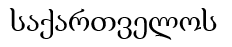
\includegraphics[scale=0.3]{images/wo_ka_word}}}'.

\highlight{\caps{EOS}.} We rephrased the task setting, since the original task introduced by \citep{Kim.2019} is not compliant with the probing task criteria \citep{Conneau.2018a}. First, we concatenate two sentences, remove punctuation and convert all words to lowercase (\textbf{NB:} Lowercasing was disabled for the German language, since this leads to many \gls{oov} nouns). Subsequently, we introduce several segments. Given the embedding of the two concatenated sentences, the classifier has to predict the correct segment where the two sentences have to be split. Thus, instead of the original binary task, we consider a multi-class classification problem. \textbf{Again, we chose the segments in a language-dependent manner:}

\begin{tabbing}
	\hspace*{3cm}\=\hspace*{4cm}\=\kill
	EN, DE, RU		\>	inflectional		\>	$[1;8], [9;12], [13;16], [17;20], [21;24], [25;28], [29;32], [33;\infty[$	\\[2mm]
	TR, KA		\>	agglutinative	\>	$[1;4], [5;8], [9;12], [13;16], [17;20], [21;\infty[$
\end{tabbing}

\highlight{\caps{SubjNum}.} We categorize sentences into \texttt{class 0}, if their subject is \textit{singular} (\texttt{Number=Singular}, cf. column \ding{186} in figure \vref{fig:ud_example}), whereas we assign \texttt{class 1} if the subject of the sentence is \textit{plural} (\texttt{Number=Plural}). Subjects could be identified by the \texttt{nsubj} tag in column \ding{188}. \textbf{We dropped sentences if their corresponding subject did not have a number tag. We also excluded sentences, if they contained more than one subject, since it is possible that each subject has a different number which renders the classification task ambiguous.}

The following tables \vref{tab:class_dist_probing_en_de}, \vref{tab:class_dist_probing_ru_tr} and \vref{tab:class_dist_probing_ka} show the class distributions for each probing task in the target languages:

% Table: Class distributions English and German
\begin{table}[h]
	\centering
	\renewcommand{\arraystretch}{1.30}
	\scalebox{0.8}{
	\begin{tabularx}{1.2\textwidth}{| l ? Y | Y | Y | Y | Y | Y | Y | Y | Y |}
		\hline
		\rowcolor{tud9c}
		\multicolumn{10}{| c |}{\textcolor{white}{\textbf{English/German}}} \\ \hline
		\rowcolor{tud9c!50}
		\textbf{Classes} & \caps{SentLen} & \caps{WC} & \caps{BiShift} & \caps{SVAgree} & \caps{SVDist} & \caps{Voice} &
			\caps{WO} & \caps{EOS} & \caps{SubjNum} \\ \hline
		\textbf{\# inst.}	& 10k/10k & 10k/10k & 10k/10k & 10k/10k & 10k/10k & 9,999/9,999 & 10k/10k & 10k/10k & 9,448/9,999 \\ \hline
		\textbf{Class 0} 	& 04.3/00.6 	& 01.0/00.6	& 50.2/49.8 	& 51.1/50.7 	& 43.5/43.6	& 61.0/50.0	& 33.3/33.3 	& 21.7/14.4 	& 75.7/50.0	\\
		\textbf{Class 1} 	& 15.9/10.4 	& 03.3/02.7	& 49.8/50.2	& 48.9/49.3	& 47.5/28.5	& 39.0/50.0	& 33.3/33.3	& 16.6/18.7	& 24.3/50.0	\\
		\textbf{Class 2} 	& 17.9/19.6	& 02.4/00.9	& 			& 			& 04.5/11.5	& 			& 33.4/33.4	& 15.5/19.3	& 			\\
		\textbf{Class 3} 	& 15.5/19.9	& 00.4/02.0	& 			& 			& 02.7/10.1	& 			& 			& 13.6/15.5	& 			\\
		\textbf{Class 4} 	& 13.5/16.0	& 00.9/02.7	& 			& 			& 01.8/06.2	& 			& 			& 10.6/11.7	& 			\\
		\textbf{Class 5} 	& 12.6/14.5	& 02.5/04.1	& 			& 			&			& 			& 			& 08.1/08.0	& 			\\
		\textbf{Class 6} 	& 06.7/07.2	& 00.3/02.0	& 			& 			& 			& 			& 			& 05.7/05.1	& 			\\
		\textbf{Class 7} 	& 04.6/04.4	& 01.3/01.0	& 			& 			& 			& 			& 			& 08.2/07.3	& 			\\
		\textbf{Class 8} 	& 08.2/06.6	& 03.4/01.0	& 			& 			& 			& 			& 			& 			& 			\\
		\textbf{Class 9} 	& 00.9/00.6	& 00.5/14.8	& 			& 			& 			& 			& 			& 			& 			\\
		\textbf{Class 10} 	& 			& 04.5/02.4	& 			& 			& 			& 			& 			& 			& 			\\
		\textbf{Class 11} 	& 			& 10.7/06.6	& 			& 			& 			& 			& 			& 			& 			\\
		\textbf{Class 12} 	& 			& 01.8/02.7	& 			& 			& 			& 			&	 		& 			& 			\\
		\textbf{Class 13} 	& 			& 00.9/02.4	& 			& 			& 			& 			& 			& 			& 			\\
		\textbf{Class 14} 	& 			& 13.3/03.9	& 			& 			& 			& 			& 			& 			& 			\\
		\textbf{Class 15} 	& 			& 01.7/05.1	& 			& 			& 			& 			& 			& 			& 			\\
		\textbf{Class 16} 	& 			& 00.8/02.2	& 			& 			& 			& 			& 			& 			& 			\\
		\textbf{Class 17} 	& 			& 01.2/02.1	& 			& 			& 			&	 		& 			& 			& 			\\
		\textbf{Class 18} 	&			& 05.0/04.7	& 			& 			& 			& 			&	 		& 			& 			\\
		\textbf{Class 19} 	& 			& 00.7/02.5	& 			& 			& 			& 			& 			& 			& 			\\
		\textbf{Class 20} 	& 			& 06.7/01.3	& 			& 			& 			& 			& 			& 			& 			\\
		\textbf{Class 21} 	& 			& 02.7/01.6	& 			& 			& 			& 			& 			& 			& 			\\
		\textbf{Class 22} 	& 			& 01.9/05.2	& 			& 			& 			& 			& 			& 			& 			\\
		\textbf{Class 23} 	& 			& 11.3/02.2	&			& 			& 			& 			& 			& 			& 			\\
		\textbf{Class 24} 	& 			& 06.2/05.7	& 			& 			& 			& 			& 			&	 		& 			\\
		\textbf{Class 25} 	& 			& 00.9/02.3	& 			& 			& 			& 			& 			& 			& 			\\
		\textbf{Class 26} 	& 			& 05.9/08.7	& 			& 			& 			& 			& 			&	 		& 			\\
		\textbf{Class 27} 	& 			& 02.0/02.4	& 			& 			& 			& 			& 			& 			& 			\\
		\textbf{Class 28} 	& 			& 03.1/01.5	& 			& 			& 			& 			& 			& 			& 			\\
		\textbf{Class 29} 	& 			& 02.5/03.1	& 			& 			& 			& 			& 			& 			& 			\\
		\hline
	\end{tabularx}}
	\caption[Class distributions for the probing tasks in English and German]
		{Class distributions for the probing tasks in English and German. One entry is given by `en/de'.}
	\label{tab:class_dist_probing_en_de}
\end{table}

% Table: Class distributions Russian and Turkish
\begin{table}
	\centering
	\renewcommand{\arraystretch}{1.0}
	\scalebox{0.8}{
	\begin{tabularx}{1.2\textwidth}{| l ? Y | Y | Y | Y | Y | Y | Y | Y | Y |}
		\hline
		\rowcolor{tud9c}
		\multicolumn{10}{| c |}{\textcolor{white}{\textbf{Russian/Turkish}}} \\ \hline
		\rowcolor{tud9c!50}
		\textbf{Classes} & \caps{SentLen} & \caps{WC} & \caps{BiShift} & \caps{SVAgree} & \caps{SVDist} & \caps{Voice} &
			\caps{WO} & \caps{EOS} & \caps{SubjNum} \\ \hline
		\textbf{\# inst.}	& 10k/10k & 10k/10k & 10k/10k & 10k/10k & 10k/2,750 & 10k/8,416 & 10k/10k & 10k/10k & 9,999/4,030 \\ \hline
		\textbf{Class 0} 	& 03.2/09.4 	& 03.8/01.6	& 48.7/49.5	& 49.9/50.6	& 42.3/20.7	& 68.0/86.2 	& 33.3/33.3	& 23.6/12.3	& 50.0/83.4 	\\
		\textbf{Class 1} 	& 16.7/37.3	& 05.0/12.6	& 51.3/50.5	& 50.1/49.4	& 40.1/39.0	& 32.0/13.8	& 33.3/33.3	& 17.8/23.7	& 50.0/16.6	\\
		\textbf{Class 2} 	& 17.4/18.9	& 02.1/00.7	& 			& 			& 09.7/16.7	& 			& 33.4/33.4	& 16.5/18.1	& 			\\
		\textbf{Class 3} 	& 16.7/11.6	& 02.9/02.1	& 			& 			& 05.3/11.8	& 			& 			& 14.1/15.6	& 			\\
		\textbf{Class 4} 	& 14.3/08.8	& 02.1/02.5	& 			& 			& 02.7/11.8	& 			& 			& 10.1/11.3	& 			\\
		\textbf{Class 5} 	& 12.4/06.7	& 03.1/02.5	& 			& 			& 			& 			& 			& 07.4/19.1	& 			\\
		\textbf{Class 6} 	& 06.8/03.1	& 02.7/00.3	& 			& 			& 			& 			& 			& 04.4/- 	& 			\\
		\textbf{Class 7} 	& 04.5/01.6	& 02.0/06.9	& 			& 			& 			& 			& 			& 06.1/- 	& 			\\
		\textbf{Class 8} 	& 07.4/02.5	& 06.3/03.9	& 			& 			& 			& 			& 			& 			& 			\\
		\textbf{Class 9} 	& 00.5/00.1	& 04.6/00.5	& 			& 			& 			& 			& 			& 			& 			\\
		\textbf{Class 10} 	& 			& 03.5/02.5	& 			& 			& 			& 			& 			& 			& 			\\
		\textbf{Class 11} 	& 			& 02.7/03.2	& 			& 			& 			& 			& 			& 			& 			\\
		\textbf{Class 12} 	& 			& 02.9/03.7	& 			& 			& 			& 			& 			& 			& 			\\
		\textbf{Class 13} 	& 			& 01.3/00.2	& 			& 			& 			& 			& 			& 			& 			\\
		\textbf{Class 14} 	& 			& 02.5/03.7	& 			& 			& 			& 			& 			& 			& 			\\
		\textbf{Class 15} 	& 			& 09.7/02.1	& 			& 			& 			& 			& 			& 			& 			\\
		\textbf{Class 16} 	& 			& 03.1/01.4	& 			& 			& 			& 			& 			& 			& 			\\
		\textbf{Class 17} 	& 			& 04.1/02.0	& 			& 			& 			& 			& 			& 			& 			\\
		\textbf{Class 18} 	& 			& 03.6/02.7	& 			& 			& 			& 			& 			& 			& 			\\
		\textbf{Class 19} 	& 			& 05.0/01.7	& 			& 			& 			& 			& 			& 			& 			\\
		\textbf{Class 20} 	& 			& 0.30/01.0	& 			& 			& 			& 			& 			& 			& 			\\
		\textbf{Class 21} 	& 			& 03.8/01.1	& 			& 			& 			& 			& 			& 			& 			\\
		\textbf{Class 22} 	& 			& 02.1/09.7	& 			& 			& 			& 			& 			& 			& 			\\
		\textbf{Class 23} 	& 			& 01.6/12.6	& 			& 			& 			& 			& 			& 			& 			\\
		\textbf{Class 24} 	& 			& 03.0/04.9	& 			& 			& 			& 			& 			& 			& 			\\
		\textbf{Class 25} 	& 			& 02.3/08.8	& 			& 			& 			& 			& 			& 			& 			\\
		\textbf{Class 26} 	& 			& 03.4/01.3	& 			& 			& 			& 			& 			& 			& 			\\
		\textbf{Class 27} 	& 			& 02.7/02.0	& 			& 			& 			& 			& 			& 			& 			\\
		\textbf{Class 28} 	& 			& 02.2/01.7	& 			& 			& 			& 			& 			& 			& 			\\
		\textbf{Class 29} 	& 			& 02.9/00.2	& 			&			& 			& 			& 			& 			& 			\\
	\hline
	\end{tabularx}}
	\caption[Class distributions for the probing tasks in Russian and Turkish]
		{Class distributions for the probing tasks in Russian and Turkish. One entry is given by `ru/tr'.}
	\label{tab:class_dist_probing_ru_tr}
\end{table}

% Table: Class distributions Georgian
\begin{table}
	\centering
	\renewcommand{\arraystretch}{1.0}
	\scalebox{0.8}{
	\begin{tabularx}{1.2\textwidth}{| l ? Y | Y | Y | Y | Y | Y | Y | Y | Y |}
		\hline
		\rowcolor{tud9c}
		\multicolumn{10}{| c |}{\textcolor{white}{\textbf{Georgian}}} \\ \hline
		\rowcolor{tud9c!50}
		\textbf{Classes} & \caps{SentLen} & \caps{WC} & \caps{BiShift} & \caps{SVAgree} & \caps{SVDist} & \caps{Voice} &
			\caps{WO} & \caps{EOS} & \caps{SubjNum} \\ \hline
		\textbf{\# inst.}	& 9,989 & 10k & 9,993 & 10k & - & 10k & 10k & 10k & - \\ \hline
		\textbf{Class 0} 	& 07.0 	& 02.1 	& 51.5 	& 50.8 	& - 	& 34.9	& 33.2 	& 26.1 	& - 	\\
		\textbf{Class 1} 	& 28.3	& 01.9	& 48.5	& 49.2 	& - 	& 65.1	& 33.3	& 28.2	& - 	\\
		\textbf{Class 2} 	& 22.3	& 04.0	&	 	& 		& 	& 		& 33.5	& 13.7	& 	\\
		\textbf{Class 3} 	& 14.8	& 08.6	&		& 		& 	& 		& 		& 08.6	& 	\\
		\textbf{Class 4} 	& 09.6	& 04.5	& 		& 		& 	& 		& 		& 06.3	& 	\\
		\textbf{Class 5} 	& 06.7	& 01.9	& 		& 		& 	& 		& 		& 17.2	& 	\\
		\textbf{Class 6} 	& 03.3	& 12.6	& 		& 		&	& 		& 		& 		& 	\\
		\textbf{Class 7} 	& 02.1	& 00.2	& 		& 		& 	& 		& 		& 		& 	\\
		\textbf{Class 8} 	& 04.8	& 09.8	& 		& 		& 	& 		& 		& 		& 	\\
		\textbf{Class 9} 	& 01.2	& 00.7	& 		& 		& 	& 		& 		& 		& 	\\
		\textbf{Class 10} 	& 		& 00.9	& 		& 		& 	& 		& 		& 		& 	\\
		\textbf{Class 11} 	& 		& 00.3	& 		& 		& 	& 		& 		& 		& 	\\
		\textbf{Class 12} 	& 		& 11.9	& 		& 		& 	& 		& 		& 		& 	\\
		\textbf{Class 13} 	& 		& 01.1	& 		& 		& 	& 		& 		& 		& 	\\
		\textbf{Class 14} 	& 		& 00.3	& 		& 		& 	& 		& 		& 		& 	\\
		\textbf{Class 15} 	& 		& 13.4	& 		& 		& 	& 		& 		& 		& 	\\
		\textbf{Class 16} 	& 		& 01.6	& 		& 		& 	& 		& 		& 		& 	\\
		\textbf{Class 17} 	& 		& 03.8	& 		& 		& 	& 		& 		& 		& 	\\
		\textbf{Class 18} 	& 		& 00.3	& 		& 		& 	& 		& 		& 		& 	\\
		\textbf{Class 19} 	& 		& 02.5	& 		& 		& 	& 		& 		& 		& 	\\
		\textbf{Class 20} 	& 		& 02.8	& 		& 		& 	& 		& 		& 		& 	\\
		\textbf{Class 21} 	& 		& 00.3	& 		& 		& 	& 		& 		& 		& 	\\
		\textbf{Class 22} 	& 		& 02.1	& 		& 		& 	& 		& 		& 		& 	\\
		\textbf{Class 23} 	& 		& 03.9	& 		& 		& 	& 		& 		& 		& 	\\
		\textbf{Class 24} 	& 		& 00.4	& 		& 		& 	& 		& 		& 		& 	\\
		\textbf{Class 25} 	& 		& 01.8	& 		& 		& 	& 		& 		& 		& 	\\
		\textbf{Class 26} 	& 		& 03.5	& 		& 		& 	& 		& 		& 		& 	\\
		\textbf{Class 27} 	& 		& 01.8	& 		& 		& 	& 		& 		& 		& 	\\
		\textbf{Class 28} 	& 		& 00.3	& 		& 		& 	& 		& 		& 		& 	\\
		\textbf{Class 29} 	& 		& 00.5	& 		& 		& 	& 		& 		& 		& 	\\
		\hline
	\end{tabularx}}
	\caption[Class distributions for the probing tasks in Georgian]
		{Class distributions for the probing tasks in Georgian.}
	\label{tab:class_dist_probing_ka}
\end{table}

% -----------------------------------------------------------------------------------------------------------------------------------------------------
% Probing Task Classifier
\subsubsection{Presentation of Classifier Architecture}
\label{sec:probing_tasks_classifier}

Researchers who deal with the evaluation of word or sentence embeddings mainly employ two types of machine learning models: \textbf{Logistic regression} and \textbf{MLPs}. Since neural networks are the state-of-the-art technique at the moment, a similar approach as in \citep{Perone.2018} is taken. \textbf{For all probing tasks, a simple feed-forward \gls{mlp} is trained using the following hyper-parameter setting:}

\begin{tabbing}
	\hspace*{4.5cm}\=\kill
	\textbf{Number of hidden layers:} 	\> 1 						\\[4mm]
	\textbf{Number of hidden units:}		\> 50 					\\[4mm]
	\textbf{Hidden layer activation:}		\> Sigmoid 				\\[4mm]
	\textbf{Dropout rate:}				\> 0.00 					\\[4mm]
	\textbf{Number of epochs:}			\> 100 					\\[4mm]
	\textbf{Optimizer:} 				\> Adam 					\\[4mm]
	\textbf{Training loss:} 			\> Categorical cross-entropy
\end{tabbing}

The input dimensionality depends on the sentence embedding algorithm which is used to encode the sentences, while the number of output nodes is determined by the number of classes considered in each probing task. Furthermore, in order to get a better and more stable estimate of the network's performance, we conduct an $n$-fold cross-validation approach. \textbf{For the evaluation, we chose $\bm{n} = 5$.}

% -----------------------------------------------------------------------------------------------------------------------------------------------------
% Chapter Summary
\subsection{Summary}
\label{sec:probing_tasks_summary}

This chapter introduced the concept of probing tasks as well as relevant tasks from the literature (cf. section \vref{sec:probing_tasks_presentation}). \citep{Conneau.2018a} organizes probing tasks for sentence embeddings into three distinct types: Surface tasks, syntactic tasks and semantic tasks. We adopted this categorization. After a brief presentation of the low-resource languages (cf. section \vref{sec:presentation_languages}), we evaluated all probing tasks w.\,r.\,t. their implementability in the target languages (cf. section \vref{sec:probing_tasks_implementability}). The surface probing tasks turned out to be the easiest to implement. Syntactic and semantic probing tasks require more linguistic knowledge about the languages and are harder to implement as a consequence. Finally, section \vref{sec:probing_tasks_implementation} gave detailed insight into the selection of probing tasks and the subsequent data generation process. For all languages, the sentences we used were taken from the \textit{\gls{ud}} tree bank corpora as well as Wikipedia, except for Georgian for which we used the \textit{\gls{gnc}} corpus as a substitute.

We implemented the following list of probing tasks: \caps{SentLen}, \caps{WC}, \caps{BiShift}, \caps{SVAgree}, \caps{SVDist} (not for Georgian), \caps{Voice}, \caps{WO}, \caps{EOS} and \caps{SubjNum} (not for Georgian). Also, the architecture of the probing task classifier was presented briefly (cf. section \vref{sec:probing_tasks_classifier}): For all probing tasks, a simple \gls{mlp} architecture is employed, where the hyper-parameters were chosen according to \citep{Perone.2018}.